%% abtex2-modelo-trabalho-academico.tex, v-1.9.6 laurocesar
%% Copyright 2012-2016 by abnTeX2 group at http://www.abntex.net.br/ 
%%
%% This work may be distributed and/or modified under the
%% conditions of the LaTeX Project Public License, either version 1.3
%% of this license or (at your option) any later version.
%% The latest version of this license is in
%%   http://www.latex-project.org/lppl.txt
%% and version 1.3 or later is part of all distributions of LaTeX
%% version 2005/12/01 or later.
%%
%% This work has the LPPL maintenance status `maintained'.
%% 
%% The Current Maintainer of this work is the abnTeX2 team, led
%% by Lauro César Araujo. Further information are available on 
%% http://www.abntex.net.br/
%%
%% This work consists of the files abntex2-modelo-trabalho-academico.tex,
%% abntex2-modelo-include-comandos and abntex2-modelo-references.bib
%%

% ------------------------------------------------------------------------
% ------------------------------------------------------------------------
% abnTeX2: Modelo de Trabalho Academico (tese de doutorado, dissertacao de
% mestrado e trabalhos monograficos em geral) em conformidade com 
% ABNT NBR 14724:2011: Informacao e documentacao - Trabalhos academicos -
% Apresentacao
% ------------------------------------------------------------------------
% ------------------------------------------------------------------------

\documentclass[
	% -- opções da classe memoir --
	12pt,				% tamanho da fonte
	openright,			% capítulos começam em pág ímpar (insere página vazia caso preciso)
	oneside,			% para impressão em recto e verso. Oposto a oneside
	a4paper,			% tamanho do papel. 
	% -- opções da classe abntex2 --
	%chapter=TITLE,		% títulos de capítulos convertidos em letras maiúsculas
	%section=TITLE,		% títulos de seções convertidos em letras maiúsculas
	%subsection=TITLE,	% títulos de subseções convertidos em letras maiúsculas
	%subsubsection=TITLE,% títulos de subsubseções convertidos em letras maiúsculas
	% -- opções do pacote babel --
	english,			% idioma adicional para hifenização
	%french,				% idioma adicional para hifenização
	%spanish,			% idioma adicional para hifenização
	brazil				% o último idioma é o principal do documento
	]{abntex2}

% ---
% Pacotes básicos 
% ---
\usepackage{lmodern}			% Usa a fonte Latin Modern			
\usepackage[T1]{fontenc}		% Selecao de codigos de fonte.
\usepackage[utf8]{inputenc}		% Codificacao do documento (conversão automática dos acentos)
\usepackage{lastpage}			% Usado pela Ficha catalográfica
\usepackage{indentfirst}		% Indenta o primeiro parágrafo de cada seção.
\usepackage{color}				% Controle das cores
\usepackage{graphicx}			% Inclusão de gráficos
\usepackage{microtype} 			% para melhorias de justificação
\usepackage{subfig}
\usepackage{float}
\usepackage{listofsymbols}

\usepackage{amsmath}
\usepackage{listings}
%\usepackage{xcolor}

%\usepackage{reledmac}


%pacote da tabela
\usepackage{multirow}
% ---
%	
% ---
% Pacotes adicionais, usados apenas no âmbito do Modelo Canônico do abnteX2
% ---
\usepackage{lipsum}				% para geração de dummy text
% ---

% ---
% Pacotes de citações
% ---
\usepackage[brazilian,hyperpageref]{backref}	 % Paginas com as citações na bibl
%\usepackage[alf]{abntex2cite}	% Citações padrão ABNT
\usepackage[alf,abnt-etal-list=0,abnt-etal-cite=3]{abntex2cite}
 
% --- 
% CONFIGURAÇÕES DE PACOTES
% --- 

% ---
% Configurações do pacote backref
% Usado sem a opção hyperpageref de backref
\renewcommand{\backrefpagesname}{Citado na(s) página(s):~}
% Texto padrão antes do número das páginas
\renewcommand{\backref}{}
% Define os textos da citação
\renewcommand*{\backrefalt}[4]{
	\ifcase #1 %
		Nenhuma citação no texto.%
	\or
		Citado na página #2.%
	\else
		Citado #1 vezes nas páginas #2.%
	\fi}%
% ---

% ---
% Informações de dados para CAPA e FOLHA DE ROSTO
% ---
\titulo{Sistema de Aquisição e Transmissão de Dados Usando Sensor de Flexão Bioinspirado}
\autor{Wederson Medeiros Silva}
\local{Belém -- Pará}
\data{2018}
\orientador{Prof. Dr. Roberto Menezes Rodriguez}
\coorientador{Prof. Dr. João Crisóstomo Weyl A. Costa}
\instituicao{
  Universidade Federal do Pará -- UFPa
  \par
  Instituto de Tecnologia -- ITEC
  \par
  Faculdade de Engenharia da Computação e Telecomunicações -- FCT}
\tipotrabalho{Trabalho de Conclusão de Curso}

% O preambulo deve conter o tipo do trabalho, o objetivo, 
% o nome da instituição e a área de concentração 
\preambulo{Trabalho de Conclusão de Curso apresentado para obtenção do
título de Bacharel em Engenharia da Computação. Instituto de Tecnologia. Faculdade de Engenharia da Computação e Telecomunicações. Universidade Federal do Pará.
}
% ---


% ---
% Configurações de aparência do PDF final

% alterando o aspecto da cor azul
\definecolor{blue}{RGB}{41,5,195}

% informações do PDF
\makeatletter
\hypersetup{
     	%pagebackref=true,
		pdftitle={\@title}, 
		pdfauthor={\@author},
    	pdfsubject={\imprimirpreambulo},
	    pdfcreator={LaTeX with abnTeX2},
		pdfkeywords={abnt}{latex}{abntex}{abntex2}{trabalho acadêmico}, 
		colorlinks=true,       		% false: boxed links; true: colored links
    	linkcolor=black,          	% color of internal links
    	citecolor=black,        		% color of links to bibliography
    	filecolor=black,      		% color of file links
		urlcolor=black,
		bookmarksdepth=4
}
\makeatother
% --- 

% --- 
% Espaçamentos entre linhas e parágrafos 
% --- 

% O tamanho do parágrafo é dado por:
\setlength{\parindent}{1.3cm}

% Controle do espaçamento entre um parágrafo e outro:
\setlength{\parskip}{0.2cm}  % tente também \onelineskip

% ---
% compila o indice
% ---
\makeindex
% ---

% ----
% Início do documento
% ----
\begin{document}

% Seleciona o idioma do documento (conforme pacotes do babel)
%\selectlanguage{english}
\selectlanguage{brazil}

% Retira espaço extra obsoleto entre as frases.
\frenchspacing 

% ----------------------------------------------------------
% ELEMENTOS PRÉ-TEXTUAIS
% ----------------------------------------------------------
% \pretextual

% ---
% Capa
% ---
\renewcommand{\imprimircapa}{
\begin{capa}

\center

\includegraphics[scale=0.4]{figures/ufpa_logo.jpg}

 { \ABNTEXchapterfont 
 UNIVERSIDADE FEDERAL DO PARÁ\\
 INSTITUTO DE TECNOLOGIA\\
 FACULDADE DE ENGENHARIA ELÉTRICA E BIOMÉDICA\\}
   \vspace*{4.0cm}
 
 { \ABNTEXchapterfont\large
   \textbf{\imprimirautor}}
   \vspace*{3.0cm}

 {\ABNTEXchapterfont\LARGE
 \textbf{\imprimirtitulo}}

 \vspace*{\fill}
 {\large\imprimirlocal}
 \par
 {\large\imprimirdata}
 \vspace*{1cm}
\end{capa}
}
% ---
% Capa
% ---
\imprimircapa
% ---

% ---
% Folha de rosto
% (o * indica que haverá a ficha bibliográfica)
% ---
%%Folha de Rosto
\makeatletter
\renewcommand{\folhaderostocontent}{
  \begin{center}

    \vspace*{0.08cm}
    {\ABNTEXchapterfont\Large
     \imprimirautor}

    \vspace*{\fill}\vspace*{\fill}
    {\ABNTEXchapterfont\LARGE
     \textbf{\imprimirtitulo}}
     \vspace*{\fill}

    \abntex@ifnotempty{\imprimirpreambulo}{
      \hspace{.45\textwidth}
      \begin{minipage}{.5\textwidth}
         \imprimirpreambulo\\    
      \end{minipage}%
       \vspace*{\fill}
    }%
    
    {\ABNTEXchapterfont\Large
     \imprimirorientadorRotulo
     \ABNTEXsectionfont~\imprimirorientador\par}
    
    {\ABNTEXchapterfont\Large
     \imprimircoorientadorRotulo
     \ABNTEXsectionfont~\imprimircoorientador}%

    \vspace*{\fill}
    {\large\imprimirlocal}
    \par
    {\large\imprimirdata}
  \end{center}
}
\makeatother

% ---
% Folha de rosto
% (o * indica que haverá a ficha bibliográfica)
% ---
\imprimirfolhaderosto*
% ---
% ---
% Inserir a ficha bibliografica
% ---

% Isto é um exemplo de Ficha Catalográfica, ou ``Dados internacionais de
% catalogação-na-publicação''. Você pode utilizar este modelo como referência. 
% Porém, provavelmente a biblioteca da sua universidade lhe fornecerá um PDF
% com a ficha catalográfica definitiva após a defesa do trabalho. Quando estiver
% com o documento, salve-o como PDF no diretório do seu projeto e substitua todo
% o conteúdo de implementação deste arquivo pelo comando abaixo:
%
% \begin{fichacatalografica}
%     \includepdf{fig_ficha_catalografica.pdf}
% \end{fichacatalografica}

\begin{fichacatalografica}
	\sffamily
	\vspace*{\fill}					% Posição vertical
	\begin{center}					% Minipage Centralizado
	\fbox{\begin{minipage}[c][8cm]{13.5cm}		% Largura
	\small
	\imprimirautor
	%Sobrenome, Nome do autor
	
	\hspace{0.5cm} \imprimirtitulo  / \imprimirautor. --
	\imprimirlocal, \imprimirdata-
	
	\hspace{0.5cm} \pageref{LastPage} p. : il. (algumas color.) ; 30 cm.\\
	
	\hspace{0.5cm} \imprimirorientadorRotulo~\imprimirorientador\\
	
	\hspace{0.5cm} \imprimircoorientadorRotulo~\imprimircoorientador\\
	
	\hspace{0.5cm}
	\parbox[t]{\textwidth}{\imprimirtipotrabalho~--~\imprimirinstituicao,
	\imprimirdata.}\\
	
	\hspace{0.5cm}
		1. Modo fantasma de segunda camada.
		2. Taxa agregada.
		3. \textit{Vectoring}.
		4. EVM.
		I. \imprimirorientador.
		II. Universidade Federal do Pará.
		III. Faculdade de Engenharia Elétrica e Biomédica.
		IV. \imprimirtitulo\\ 		
	\end{minipage}}
	\end{center}
\end{fichacatalografica}
% ---
% ---

% ---
% Inserir folha de aprovação
% ---

% Isto é um exemplo de Folha de aprovação, elemento obrigatório da NBR
% 14724/2011 (seção 4.2.1.3). Você pode utilizar este modelo até a aprovação
% do trabalho. Após isso, substitua todo o conteúdo deste arquivo por uma
% imagem da página assinada pela banca com o comando abaixo:
%
% \includepdf{folhadeaprovacao_final.pdf}
%
\begin{folhadeaprovacao}

  \begin{center}
    {\ABNTEXchapterfont\large\imprimirautor}

    \vspace*{\fill}\vspace*{\fill}
    \begin{center}
      \ABNTEXchapterfont\bfseries\Large\imprimirtitulo
    \end{center}
    \vspace*{\fill}
    
    \hspace{.45\textwidth}
    \begin{minipage}{.5\textwidth}
        \imprimirpreambulo
    \end{minipage}%
    \vspace*{\fill}
   \end{center}
        
   Trabalho aprovado. \imprimirlocal, 24 de dezembro de 2018:

   Conceito: .
   
   \assinatura{\textbf{\imprimirorientador} \\ Orientador} 
   \assinatura{\textbf{\imprimircoorientador} \\ Coorientador}
   \assinatura{\textbf{Prof. Dr. Gilvan Borges} \\ Convidado 1}
  % \assinatura{\textbf{Prof. Dr. Somebody else} \\ Convidado 2}
   %\assinatura{\textbf{Professor} \\ Convidado 3}
      
   \begin{center}
    \vspace*{0.5cm}
    {\large\imprimirlocal}
    \par
    {\large\imprimirdata}
    \vspace*{1cm}
  \end{center}
  
\end{folhadeaprovacao}
% ---

% ---
% Dedicatória
% ---
\begin{dedicatoria}
   \vspace*{\fill}
   \centering
   \noindent
   \textit{ Este trabalho é dedicado...} \vspace*{\fill}
\end{dedicatoria}
% ---

% ---
% Agradecimentos
% ---
\begin{agradecimentos}
Agradeço ao Professor Dr. ...
\end{agradecimentos}
% ---
% ---

% ---
% Epígrafe
% ---
\begin{epigrafe}
    \vspace*{\fill}
	\begin{flushright}
		\textit{``Não vos amoldeis às estruturas deste mundo, ...)}
	\end{flushright}
\end{epigrafe}
% ---

% ---
% RESUMOS
% ---

% resumo em português
\setlength{\absparsep}{18pt} % ajusta o espaçamento dos parágrafos do resumo
\begin{resumo}
%\setlength{\parindent}{1.5cm}
%\indent
%\hangindent=3.7cm
\hspace{1.5cm}O modo \textit{fronthaul} de redes 5G ...
	
 \textbf{Palavras-chaves}: Modo fantasma. 
\end{resumo}

% resumo em inglês
\begin{resumo}[Abstract]
 \begin{otherlanguage*}{english}
\hspace{1.5cm}Phantom mode has...

   \vspace{\onelineskip}
 
   \noindent 
   \textbf{Keywords}: Phantom mode. 
 \end{otherlanguage*}
\end{resumo}


% ---
% inserir lista de ilustrações
% ---
\pdfbookmark[0]{\listfigurename}{lof}
\listoffigures*
\cleardoublepage
% ---

% ---
% inserir lista de tabelas
% ---
\pdfbookmark[0]{\listtablename}{lot}
\listoftables*
\cleardoublepage
% ---

% ---
% inserir lista de abreviaturas e siglas
% ---
%\imprimirlistadesiglas
\begin{siglas}

	\item[AM]\textit{Amplitude Modulation}
	\item[I]Corrente
	\item[IDE]\textit{Integrated Development Interface}
	\item[$k\Omega$]\textit{Kiloohm}
	\item[LED]\textit{Light-Emitting Diode}
	\item[LiPo]\textit{Lithium-ion Polymer}
	\item[$mAh$]\textit{Milliampere Hour}
	\item[$Mhz$]\textit{Megahertz}
	\item[mm]\textit{Millimeter}
	\item[PCI]Placa de Circuito Impresso
	\item[PVC]\textit{Polyvinyl Chloride}	
	\item[R]Resistência
	\item[RF]\textit{Radio Frequence}
	\item[V]Tensão	
	
\end{siglas}
% ---

% ---
% inserir lista de símbolos
% ---
\begin{simbolos}
  \item[$\alpha$] Contante de atenuação
  \item[$\beta$] Contante de fase
  \item[$\gamma$] Contante de propagação
  \item[$\Gamma_{L}$] Coeficiente de reflexão na carga
  \item[$\delta$] Constante da restrição de potência transmissão
  \item[$\Delta_f$ ] Subcanais ou tons em Hz
  \item[$ \Gamma $]  Gap de $RSIR$
  \item[$ \Lambda $] Matriz que contém os elementos da diagonal principal de $\mathbf{H}$
  \item[$\rho$] Máscara espectral utilizada pelo sistema DSL
  %  \item[
  \item[${\sigma}^{2}$]  Densidade espectral de potência potência do ruído Gaussiano branco aditivo
\end{simbolos}
% ---

% ---
% inserir o sumario
% ---
\pdfbookmark[0]{\contentsname}{toc}
\tableofcontents*
\cleardoublepage
% ---



% ----------------------------------------------------------
% GUIA DAYNARA
% ----------------------------------------------------------
%{\color{green}
%1- Introdução 
%
%Seção 1: Contexto:
%
%	-Contexto da tecnologia, contendo um histórico das evoluções ADSL – VDSL – G. Fast 
%	
%	-Apontar limitações dos sistemas em relação a transmissão (taxa agregada)
%	
%	-Quais as soluções que estão sendo investigadas
%	
%	-Uma das soluções é buscar modos de transmissão alternativos
%	
%	-Modo fantasma, split-pair e wire-shield 
%	
%Seção 2: Trabalhos relacionados (até onde eles abordaram)
%
%Seção 3: *Motivação:
%Por que pesquisar esta área e esse tema de modos alternativos de transmissão, onde poderia ser aplicados (5G, XG.), etc.;
%
%Seção 4: *Justificativa:
%Quais são exatamente as contribuições, o que eu fiz a mais em relação ao que já existe.
%
%Seção 6:*Objetivos
%
%Seção 5:*Resumo da metodologia
%
%Seção :*organização do trabalho
%}
%{\color{red}


% ----------------------------------------------------------
% ELEMENTOS TEXTUAIS
% ----------------------------------------------------------
\textual

\chapter{Introdução} % ou \input{arquivoexterno}
		
		Contextualização; Estado da arte (se tiver); Motivação; O que vai fazer; Metodologia; O que terá no resto do documento;


	% --------------------- 
	%	REFERENCIAL TEÓRICO	
	% --------------------- 
	
	\chapter{Referencial Teórico}

		\section{Movimentação dos dedos}
		Na mão, os tendões funcionam como cordas que conectam os músculos do antebraço aos ossos da mão. Nos dedos, os tendões passam por dentro de uma série de polias, que formam uma espécie de túnel. Isso permite manter os tendões próximos aos ossos da mão, aumentando a força nos dedos e diminuindo o gasto de energia. Ao movimentar o dedo, o músculo se contrai para que o tendão deslize por entre as polias. \cite{drricardocirurgiao}
 
		\begin{figure}[h!]
			\centering
  		\caption{Movimento do dedo através do tendão.}
  		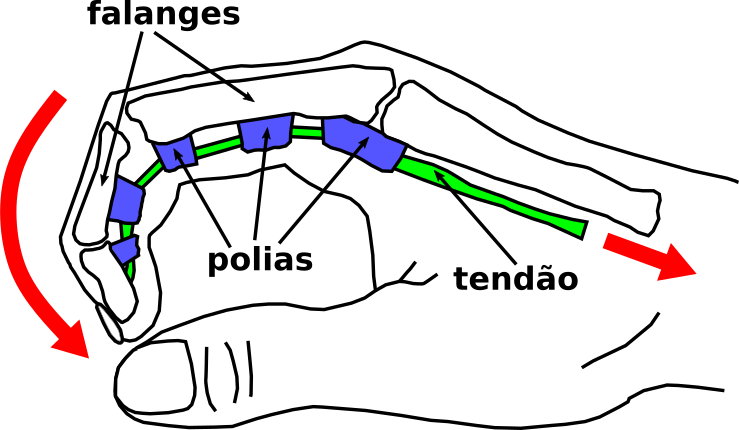
\includegraphics[scale=0.5]{./figures/hand-tendon-flex1.png}
  		\label{Fig:hand-tendon-flex1}
		\end{figure}


		\section{Sensor Flex}

		Sensores de flexão, mais conhecidos como sensores flex, são resistores analógicos que trabalham como divisores de tensão analógicos. Dentro desses sensores existem elementos resistivos de carbono junto a um fino substrato flexível. Mais carbono significa menos resistência. Quando o substrato é torcido o sensor produz uma resistência relativa ao raio da torção. \cite{solanki2013sign}.

	\begin{figure}[!h]
		\centering
		\caption{Sensor de Flexão.}
		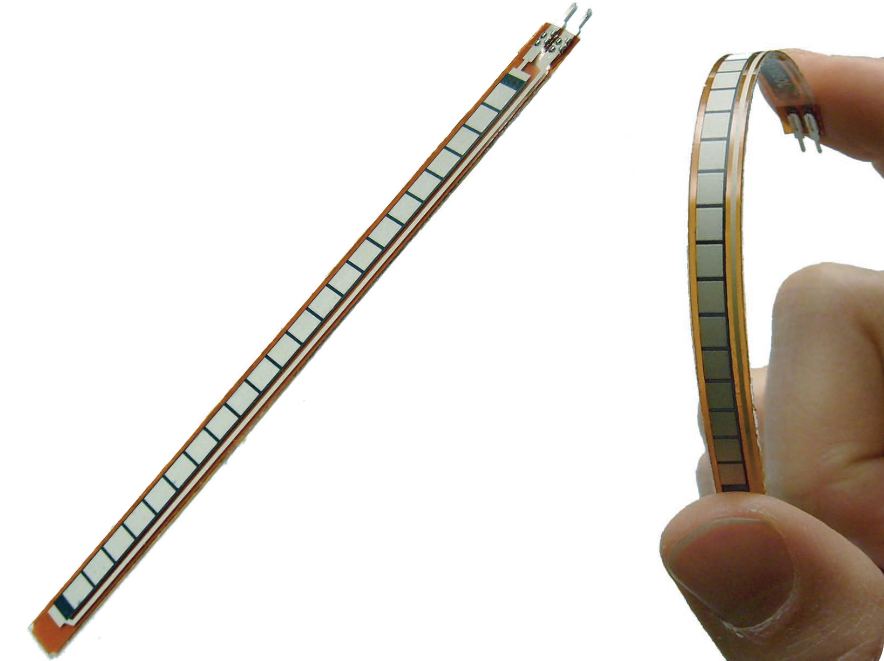
\includegraphics[width=7cm,keepaspectratio=true]{./figures/flex-sensor1.png}
		\fonte{Site Sparkfun.}%
		\label{Fig:flex-sensor1}
	\end{figure}

		\section{Potenciômetro}
		O potenciômetro é um componente eletrônico que permite, através do giro do seu eixo, a variação da resistência entre seus terminais. Eles são constituídos por um elemento de resistência, que pode ser de carbono ou fio de nicromo, sobre o qual corre uma lingueta, denominada cursor. Dentre as características do potenciômetro estão o valor máximo de sua resistência, seu número de voltas, seu grau máximo de giro (aproximado) e se ele é do tipo linear ou logarítmico \cite{ncb2012eletronicabasica}.


		\begin{figure}[h!]
			\centering
  		\caption{Funcionamento do potenciômetro linear.}
  		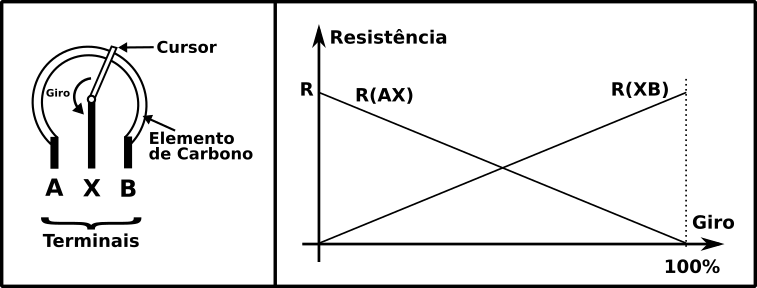
\includegraphics[width=12cm]{./figures/potentiometer1.png}
			\fonte{Modificado de~\cite{ncb2012eletronicabasica}.}
  		\label{Fig:potentiometer1}
		\end{figure}

		Segundo a lei de Ohm ($V = R.I$), dada uma corrente constante, ao variar a resistência teremos uma variação da tensão. Sendo assim, ao girar o eixo do potenciômetro, dependendo do sentido do giro, perceberemos um aumento ou diminuição da tensão naquele ponto. Partindo de um ponto extremo com resistência mínima até o outro ponto extremo no qual a resistência deverá ser a máxima característica do componente.


		\section{Arduino}
		O Arduino é uma plataforma eletrônica de código aberto que é baseada em \textit{hardware} e \textit{software} fáceis de usar. As placas Arduino são capazes de ler entradas como o acionamento de um sensor, o pressionamento de um botão, ou uma mensagem do Twitter. Pode transformar essas entradas em saídas como a ativação de um motor, o acendimento de um LED ou até a publicação de algo online. O comportamento dessa placa pode ser programado usando sua IDE (\textit{Integrated Development Interface}), que por sua vez, envia as instruções necessárias para o microcontrolador instalado na placa.\cite{arduinosite}
		
		\begin{figure}[h!]
			\centering
			\caption{Placa Arduino modelo Nano.}
  		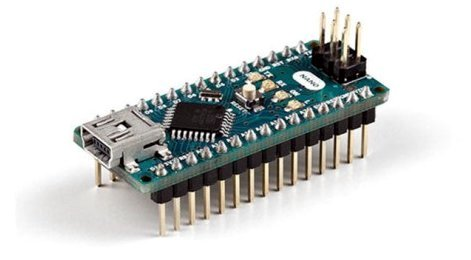
\includegraphics[width=12cm]{./figures/arduino-nano1.jpg}
  		\label{Fig:arduino-nano1}
			\fonte{Produzido pelo autor.}
		\end{figure}

		\section{Módulo RF 433 Mhz}
		O módulo de RF (Rádio Frequência) 433 Mhz é composto por um par que contém um transmissor e um receptor, opera com modulação AM (\textit{Amplitude Modulation}) e é uma alternativa para projetos de baixo custo que queiram usar comunicação sem fio entre microcontroladores Arduino ou outros. O par de módulos pode alcançar até 200 metros sem obstáculos, usando antenas e dependendo da tensão aplicada.\cite{institutodigitalrf}


		\begin{figure}[h!]
			\centering
			\caption{Módulos RF transmissor (esq.) e receptor (dir.).}
  		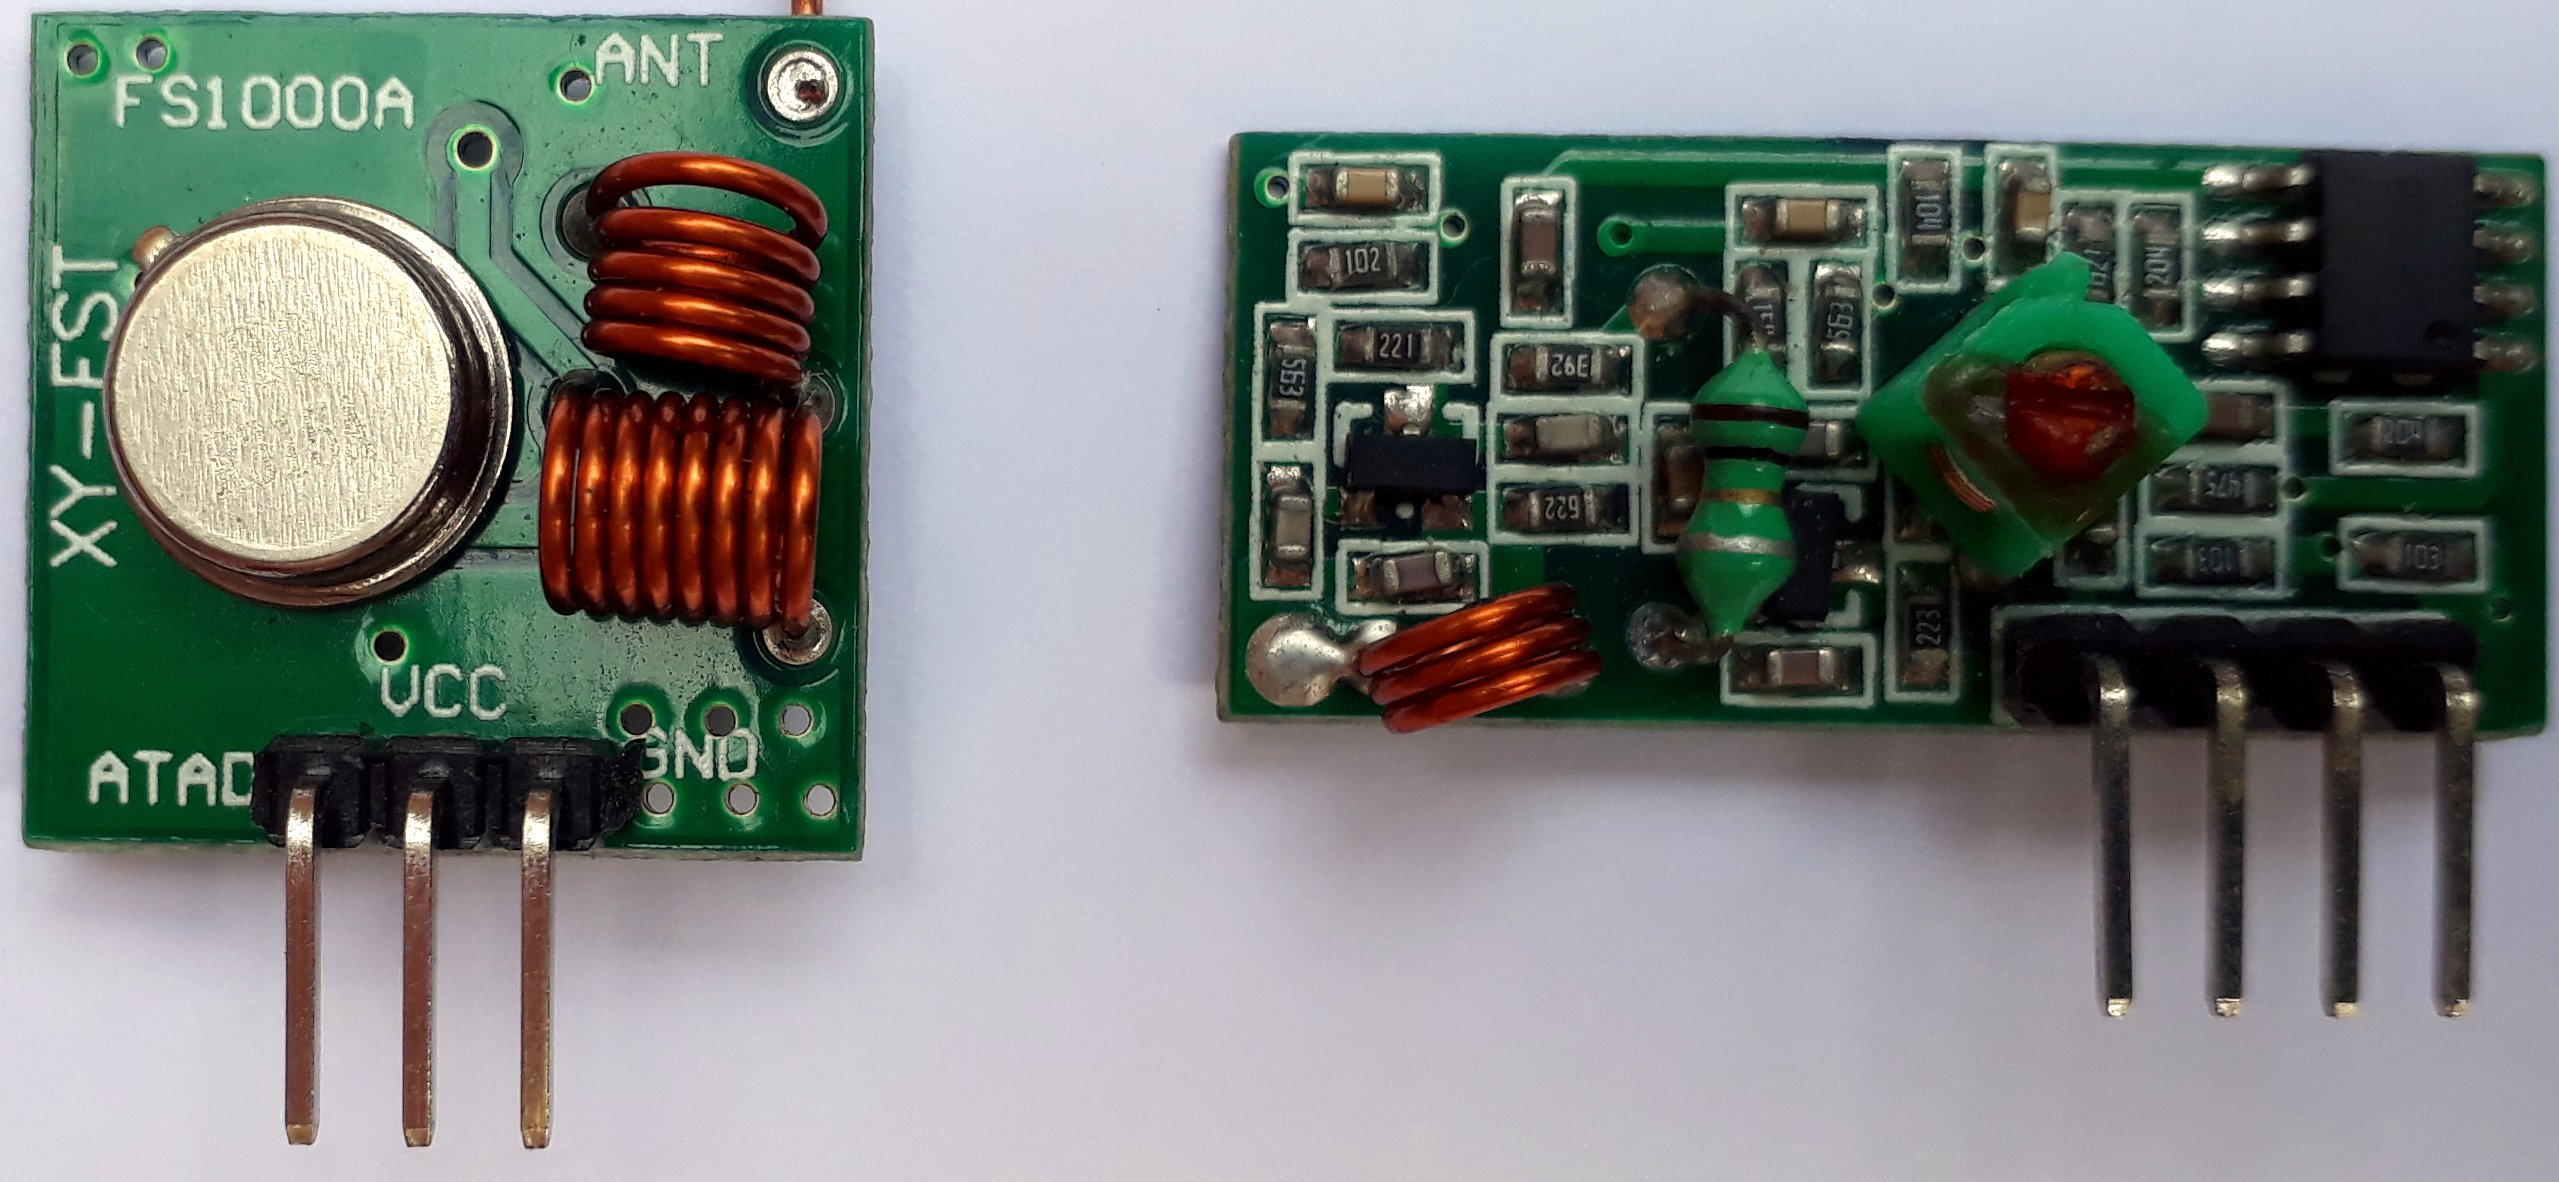
\includegraphics[width=12cm]{./figures/tx-rx1.jpg}
  		\label{Fig:tx-rx1}
			\fonte{Produzido pelo autor.}
		\end{figure}


%+++++++++++++++++++++++++++++++++++++++++++++++++++++++++++++
%
%			TRABALHO PROPRIAMENTE DITO	
%
%+++++++++++++++++++++++++++++++++++++++++++++++++++++++++++++
	
	\chapter{Trabalho Propriamente Dito}

		\section{Introdução}
		
		O capítulo a seguir está organizado em 5 seções. Na primeira delas explica-se a movimentação mecânica do sistema e como as posições de flexão e extensão dos dedos são obtidas pelo microcontrolador. A segunda aborda a programação do microcontrolador, mais precisamente o tratamento dos dados recebidos a partir dos potenciômetros. A terceira seção explica os ajustes realizados em software. A quarta explica o protocolo criado para controlar um carrinho via rádio frequência. A quinta e última seção explica como o sistema foi montado.



		\section{Mecânica Bioinspirada}

			\subsection{Transdutor de Flexão}

		Como foi explicitado previamente, através dos tendões, têm-se a movimentação dos dedos na mão. Baseado nessa biomecânica, foi desenvolvido um sistema mecânico semelhante, com o intuito de criar um transdutor de flexão de dedos atrelado a um microcontrolador. 

		No sistema biomecânico, resumidamente, uma das extremidades do tendão está presa nas falanges do dedo enquanto sua extensão desliza por dentro de polias até o músculo. No sistema desenvolvido, cada transdutor é composto por uma linha de náilon presa ao dedo da luva, guiada através de pequenos segmentos plásticos até o cursor de um potenciômetro. A figura \ref{Fig:bio-and-system} demonstra um pouco dos dois sistemas.


	\begin{figure}[!htb]
		 \centering
		 \caption{(a) Sistema biomecânico e (b) sistema desenvolvido.} 
		 \subfloat[]
		 {
			 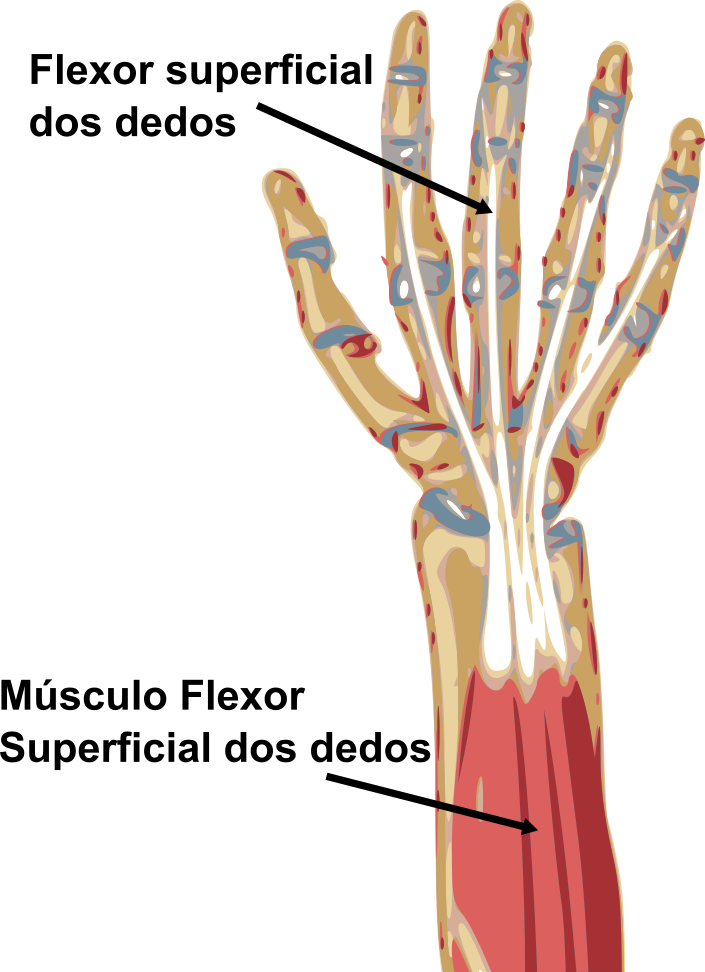
\includegraphics[width=5cm,keepaspectratio=true]{./figures/moore-biomechanic.png}
		 }
		 \centering
		 \subfloat[]
		 { 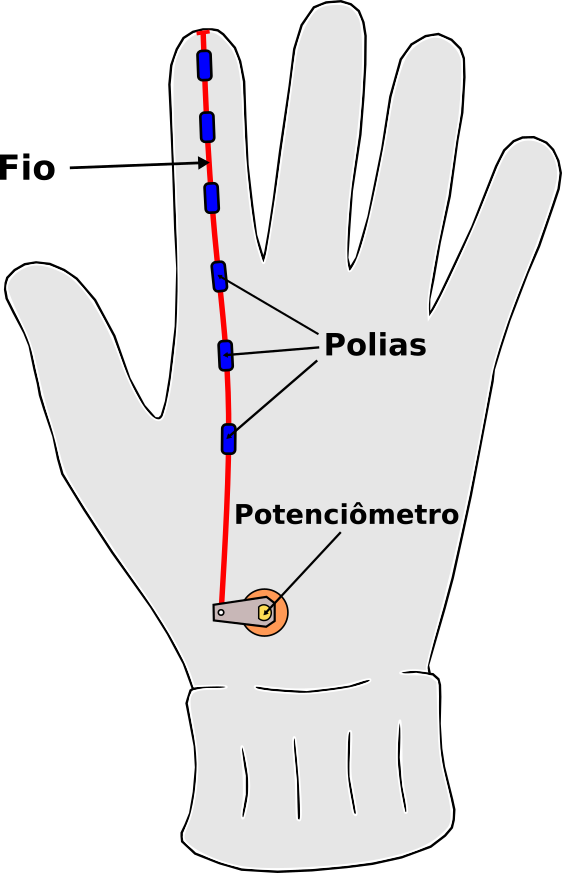
\includegraphics[width=4cm,keepaspectratio=true]{./figures/glove-wire-pot2.png}
		 }
		 \label{Fig:bio-and-system}
		 \fonte{(a) Adaptado de \cite{moore2013clinically} e (b) produzido pelo autor.}
	\end{figure}

		Logo no inicio do trabalho, foi formulada a hipótese de que poderia haver a movimentação de um fio durante a flexão de um dedo. Portanto foi realizado um experimento para verificar tal hipótese. 
		
		Sendo assim, o primeiro passo foi, com a mão inicialmente extendida com o dorso voltado para cima, uma das pontas de um fio foi presa na extremidade de um dos dedos. O local da outra ponta do fio foi marcada no dorso mão. Como é demonstrado na figura \ref{Fig:hand-wire-steady-and-flex} (a).

			Após a flexão dos dedos, verificou-se que o fio se movimentou em uma direção e criou um deslocamento (d) do fio em relação ao ponto marcado, mostrado na figura \ref{Fig:hand-wire-steady-and-flex} (b). Esse experimento validou a hipótese formulada previamente. 

%\begin{figure}[H]
%	\caption{Cabo de pares trançados.}
%	\centering
%	\subfloat[Sem blindagem]{
%		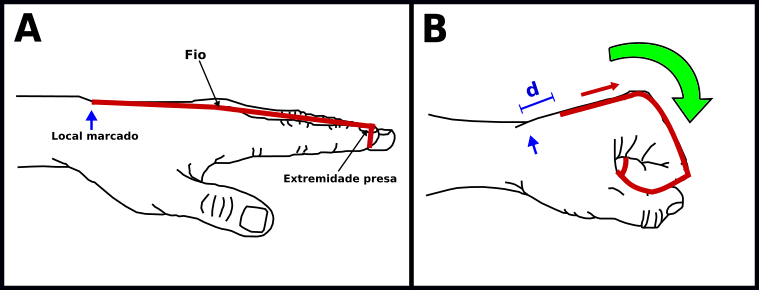
\includegraphics[width=7cm,keepaspectratio=true]{./figures/hand-wire-flex1.png}
%		\label{Fig:UTP}}
 
%	\centering
%	\subfloat[Com blindagem]{
%		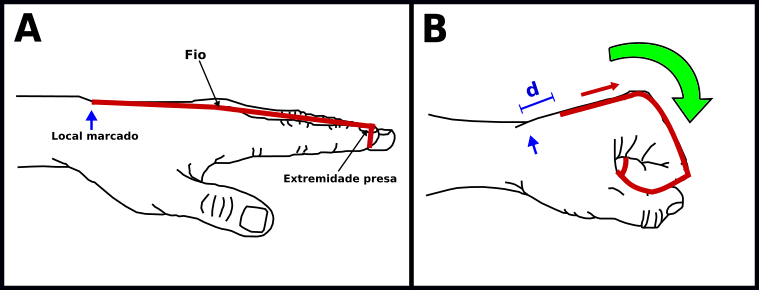
\includegraphics[width=7cm,keepaspectratio=true]{./figures/hand-wire-flex1.png}
%		\label{Fig:STP}}
%	\fonte{.}%
%	\label{Fig:Par}
%\end{figure}

\begin{figure}[!htb]
   \centering
   \caption{ (a) Mão em posição inicial e (b) Mão após flexão.}
   \subfloat[]
   {
     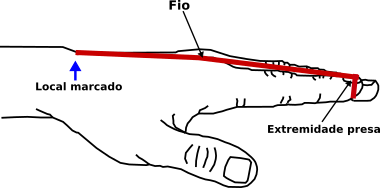
\includegraphics[width=8cm,keepaspectratio=true]{./figures/hand-wire-steady1.png}
   }
   \centering
   \subfloat[]
   { 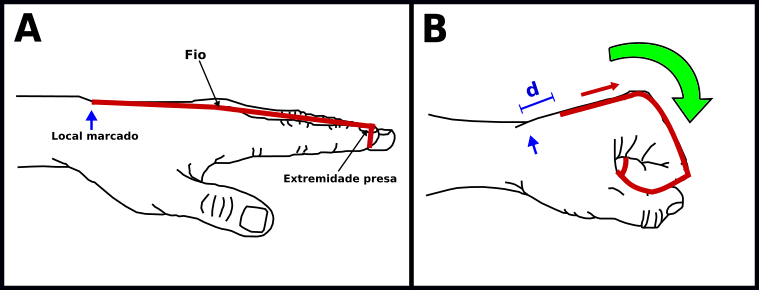
\includegraphics[width=6cm,keepaspectratio=true]{./figures/hand-wire-flex1.png}
   }
   \label{Fig:hand-wire-steady-and-flex}
   \fonte{Produzido pelo autor.}
 \end{figure}


		\subsection{Adaptação na Luva}

%			Após examinar o movimento descrito acima, foi decidido embarcar todo o sistema em uma luva. Fios foram presos às extremidades dos dedos da luva, passando por polias plásticas que servem de guias. Na extremidade oposta, os fios são conectados à pequenos potenciômetros que variam de acordo com o sentido do movimento de cada fio. Figura \ref{Fig:glove-and-transmitter1}. Sendo assim, ao final, para os cinco dedos da mão, serão necessários cinco fios e cinco potenciômetros.


%		\begin{figure}[h!]
%			\centering
%			\caption{Captação do sinal.}
%  		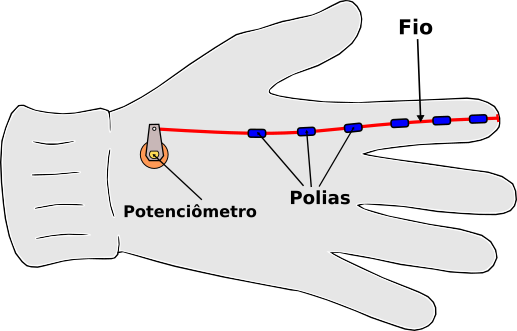
\includegraphics[scale=0.7]{./figures/glove-wire-pot1.png}
%  		\label{Fig:glove-and-transmitter1}
%			\fonte{Produzido pelo autor.}
%		\end{figure}


%		\subsection{Flexão e Extensão dos Dedos}

		Após as polias e o fio de náilon serem devidamente embarcados na luva juntamente ao potenciõmetro, com a mão extendida e mantendo o fio de náilon tensionado, ao flexionar o dedo, o fio é puxado pela ponta do dedo e com isso o cursor do potênciometro é variado. Porém, após a flexão do dedo, ao realizar o movimento inverso (extenção), não há força que movimente o fio de náilon e nem o cursor do potenciômetro de volta às suas posições iniciais.
		
		Para possibilitar que o sistema retorne à sua posição inicial, um pequeno elástico foi instalado junto ao cursor do potenciômetro. Usando o elástico durante o movimento de flexão, o cursor gira e estica o elástico. Estando esticado, o elástico busca retomar sua posição de equilíbro realizando uma força contrária para girar o cursor de volta à sua posição inicial. Figura \ref{Fig:glove-flex-and-extend2} (a).
		
		Quando há o movimento de extensão do dedo, o elástico puxa o cursor do potenciômetro girando-o em sentido inverso ao que ocorreu durante a flexão. Isso acontece enquanto o elástico estiver esticado o suficiente para exercer força sobre o cursor do potenciômetro. Demonstrado na figura \ref{Fig:glove-flex-and-extend2} (b)
		

	\begin{figure}[!htb]
		 \centering
		 \caption{ Movimentos da luva de (a) flexão e (b) extensão.} 
		 \subfloat[]
		 {
			 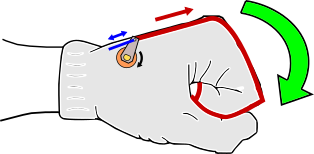
\includegraphics[width=6.5cm,keepaspectratio=true]{./figures/glove-wire-flex2.png}
		 }
		 \centering
		 \subfloat[]
		 { 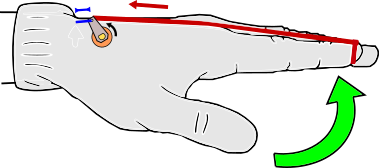
\includegraphics[width=7.5cm,keepaspectratio=true]{./figures/glove-wire-extend2.png}
		 }
		 \label{Fig:glove-flex-and-extend2}
		 \fonte{Produzido pelo autor.}
	\end{figure}


	
		\section{Programação do microcontrolador}

		\subsection{Digitalização do sinal}

		Na luva, além do transdutor, há um microcontrolador que capta os movimentos do potenciômetro e os digitaliza. O sinal chega em portas analógicas de um Arduino modelo Nano que converte a variação de tensão do potenciômetro em valores inteiros entre 0 e 1023. 

		Para facilitar a abordagem do trabalho, cada dedo da luva e seu respectivo potenciômetro é representado por um número de 1 a 5, começando pelo dedo mínimo (1) até o polegar (5). 
	 Também foram definidas duas posições principais para analisar o movimento dos dedos. Posição A: Quando todos os dedos estiverem estendidos. Posição B: Quando todos os dedos estiverem flexionados. Algo semelhante à figura \ref{Fig:glove-flex-and-extend2}.

	 	Para cada posição, o potenciômetro apresenta uma média de valores digitais. Por exemplo, quando o dedo mínimo (1) está extendido (posição A), seu respectivo potenciômetro apresenta valores em torno 191. Quando esse dedo é totalmente flexionado (posição B) seus valores ficam em torno de 616. %Então para calcular o deslocamente temos:

%	\begin{equation}
%		\begin{split}
%			\Delta Pos 	& = Pos 2 	- 	Pos 1 	\\
%									& = 558 		- 	157			\\
%						 			& = +383
%		\label{Eq:Desloca1}
%		\end{split}
%	\end{equation}

		Porteriormente, para diminuir o tamanho da mensagem a ser enviada, o valor digital apresentado pelo potenciômetro é remapeado para uma faixa de valores inteiros que representam posições inteiras entre 0 e 9. Quando os valores de todos os potenciômetros são remapeados, eles são concatenados em um único número de 5 dígitos, no qual cada dígito representa cada um dos cinco dedos da esquerda para a direita. 
		
		Por exemplo, em uma mensagem "69071" o dedo 1 (mínimo) está na posição 6, o dedo 2 (anelar) está na posição 9 e assim sucessivamente até o dedo 5 (polegar) que está na posição 1.
		
		
		\subsection{VirtualWire}

		VirtualWire é uma biblioteca de comunicação para Arduino que possibilita vários Arduinos se comunicarem usando transmissores e receptores RF de baixo custo. Essa biblioteca permite o envio de mensagens curtas, sem endereçamento, retransmissão ou confirmação, como se fosse uma espécie de protocolo UDP (\textit{User Datagram Protocol}), usando modulação ASK (\textit{Amplitude Shift Keying}) \cite{virtualwiremanual}. 

		O uso dessa biblioteca nos códigos da IDE do Arduino, permite abstrair tratamentos de envio e recebimento de dados tais como, sincronização de padrões, balanceamento de bits 0 e 1, e checagem de erros \cite{virtualwirepjrc}. Dessa forma, para enviar e receber mensagens, basta seguir os padrões de entrada e saída das funcões descritas na biblioteca.

		No código embarcado no microcontrolador da luva foram definidos, segundo os parâmetros da biblioteca, o pino do transmissor RF, a taxa de transmissão e o tamanho da mensagem a ser enviada. Porém, antes de efetivamente enviar a mensagem é preciso convertê-la em uma string que logo em seguida será transformada em um vetor de char, que é o formato de dado aceito pela função de envio.

		Uma das formas de converter valores inteiros em string é concatenar o valor inteiro com uma string \cite{arduinostringadd}. Por isso, no código desenvolvido, uma string vazia é somada aos valores inteiros remapeados dos potenciômetros. Com isso, os valores serão concatenados e transformados em uma string ao mesmo tempo. Essa string então é transformada em um vetor de char usando a função "toCharArray" antes de ser enviada. Este processo está descrito resumidamente no pseudocódigo abaixo.		

\lstset{language=C++,
%                basicstyle=\ttfamily,
                keywordstyle=\color{blue}\ttfamily,
                stringstyle=\color{green}\ttfamily,
                commentstyle=\color{red}\ttfamily,
								basicstyle=\footnotesize,
                morecomment=[l][\color{magenta}]{\#}
}
\begin{lstlisting}
	// Inicia variaveis
	string vazia = ""
	string mensagem = ""
	
	// Recebe as posicoes de cada dedo
	int dedo1 = posicao_dedo1;
	int dedo2 = posicao_dedo2;
	int dedo3 = posicao_dedo3;
	int dedo4 = posicao_dedo4;
	int dedo5 = posicao_dedo5;

	// Concatena os inteiros e os transforma em string
	mensagem = vazia + dedo1 + dedo2 + dedo3 + dedo4 + dedo5;

	// Converte a string em um vetor de char
	mensagem = mensagem.toCharArray;

	// Envia o vetor de char
	vw_send(mensagem);

\end{lstlisting}

				
%		Um resumo do processo de digitalização e envio é demonstrado na figura \ref{Fig:get-and-send}.


%		\begin{figure}[h!]
%			\centering
%			\caption{Digitalização e envio do sinal}
%  		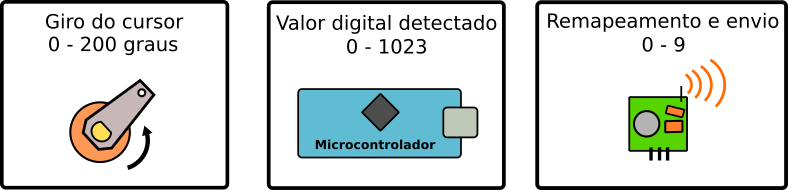
\includegraphics[width=12cm]{./figures/get-and-send.png}
% 		\label{Fig:get-and-send}
%			\fonte{Produzido pelo autor.}
%		\end{figure}



		\section{Ajustes}
		
		\subsection{Introdução}

		Quando os dedos estão em um mesmo grau de flexão, na grande maioria das vezes, os valores detectados para cada dedo são diferentes. Quando a luva está em posição A (extendida), por exemplo, o valor detectado no dedo mínimo (1) fica em torno de 192, enquanto que o anelar (2) apresenta, ao mesmo tempo, um valor em torno de 141.	
		
		Além do mais, devido à posição em que cada potenciômetro foi soldado na placa embarcada, alguns potênciômetros apresentam deslocamentos positivos ou negativos para um mesmo movimento. 
	
		\subsection{Deslocamento e número de posições}

		Para descobrir os valores de deslocamento, cada potenciômetro teve seu valor digital anotado para as posições A e B, que posteriormente foram usados na equação \ref{Eq:Desloca1}:

	\begin{equation}
			\Delta Pos 	= Pos B 	- 	Pos A
		\label{Eq:Desloca1}
	\end{equation}

		Usando o módulo de $\Delta Pos$ é possível calcular o número de posições detectáveis partindo da Posição A até a Posição B, através da equação \ref{Eq:NPos1}:

	\begin{equation}
			NPos = |\Delta Pos| + 1
		\label{Eq:NPos1}
	\end{equation}

		A tabela \ref{Tab:deltapos} mostra os valores obtidos e calculados para cada um dos cinco potenciômetro no deslocamento da posição A para a posição B.


	\begin{table}[H]
  	\centering
		\caption{Valores de A para B}
    \begin{tabular}{c|cccc}
      \midrule
			Dedo	& PosA	& PosB	& $\Delta$Pos	& NPos	\\
      \midrule
			1 		& 191 	& 616 	& 		+425 		&	426		\\
			2 		& 140 	& 609 	& 		+469 		&	470		\\
			3 		& 774 	& 360 	& 		-414 		&	415		\\
			4 		& 728 	& 475 	& 		-253 		&	254		\\
			5 		& 670 	& 367 	& 		-303 		&	304		\\      
      \midrule
    \end{tabular}
    \label{Tab:deltapos}
    \fonte{Produzido pelo autor}
	\end{table}
		
		Quanto maior for o valor de NPos na tabela \ref{Tab:deltapos}, mais preciso será o sensoriamento do dedo. Sendo assim, o anelar (2) é o dedo com maior potencial de sensoriamento, enquanto que o indicador (4) possui menor potencial.

	\subsection{Remapeamento}

	 Com o intuito de diminur o tamanho da mensagem a ser enviada pelo transmissor de rádio frequência, foi definido que cada potenciômetro teria apenas 10 níveis de deslocamento representados durante a transmissão. Dessa forma, em uma mensagem numérica, bastaria 1 dígito para representar a posição atual do dedo.

	 Junto a isso, para diminuir a complexidade do protocolo de comando, foi decidido que não haveriam deslocamentos negativos. Algo que acontece nos dedos 3, 4 e 5 durante o deslocamente de A para B.

	 Para se adequar aos requisitos descritos, no código embarcado foi usada a função "map", que permite remapear uma faixa de valores em outra menor. Usando tal função, a faixa de entrada que inicialmente poderia variar entre 0 e 1023, foi remapeada para variar entre 0 e 9 valores inteiros. 
	 
	 Além do mais, a função map também permite inverter a saída, de uma forma que os valores de entrada que variam de 1023 a 0 (decrescente) passarão a variar de 0 a 9 (crescente). Este último requisito, permite eliminar os deslocamentos negativos.

	 Usando as equações \ref{Eq:Desloca1} e \ref{Eq:NPos1}, os valores digitais remapeados (R) foram adicionados à tabela \ref{Tab:deltapos}, criando a tabela \ref{Tab:deltaremap}:


	\begin{table}[H]
  	\centering
		\caption{Valores de A para B e remapeados (R).}
    \begin{tabular}{c|cc|cc|cc|cc}
      \midrule
			Dedo	&\multicolumn{2}{c}{PosA	(RA)} 	&\multicolumn{2}{c}{PosB (RB)}	&\multicolumn{2}{c}{$\Delta$Pos	($\Delta$R)}	&\multicolumn{2}{c}{NPos	(NR)}	\\
      \midrule
			1 		& 191 & (1)		& 616 & (5)		& 		+425 & (+4)		&			425	& (5)		\\
			2 		& 140 & (1)		& 609 & (5)		& 		+469 & (+4)		&			469 &	(5)		\\
			3 		& 774 & (3)		& 360 & (6)		& 		-414 & (+3)		&			414	& (4)		\\
			4 		& 728 & (3)		& 475 & (5)		& 		-253 & (+2)		&			253	& (3)		\\
			5 		& 670 & (4)		& 367 & (6)		& 		-303 & (+2)		&			303 &	(3)		\\      
      \midrule
    \end{tabular}
    \label{Tab:deltaremap}
    \fonte{Produzido pelo autor}
	\end{table}
	

		
		\section{Protocolo de comunicação}

		\subsection{Introdução}

		Através de um transmissor de rádio frequência, a o sistema embarcado na luva envia constantemente mensagens de 5 dígitos que indicam a posição de cada um dos cinco dedos. Para receber esse sinal, é preciso usar um módulo receptor de rádio frequência compatível com o transmissor. 
		
		Um sistema receptor foi embarcado em um carrinho usando um segundo microcontrolador Arduino modelo Nano e um módulo receptor RF. Esse carrinho funciona com motores DC (\textit{Direct Current}) e todo o sistema é alimentado por uma bateria LiPo. 

		Para possibilitar o controle, conjuntos pré-definidos das posições dos dedos correspondem a movimentos que devem ser executados pelo carrinho.
		
		\subsection{Posições e movimentos}

		Como foi explicitado anteriormente, a mensagem transmitida pela luva consiste em um conjunto de 5 dígitos no qual cada dígito indica a posição de um respectivo dedo. Na mensagem, o primeiro dígito da esquerda indica a posição do dedo 1, que é o dedo mínimo. O segundo dígito indica a posição do dedo 2, ou seja, o dedo anelar. Essa lógica segue até o quinto dígito que representa a posição do dedo polegar.

		Cinco comandos foram definidos para o carrinho, ir para frente, ir para trás, girar para a esquerda, girar para a direita e parar. Com o intuito de controlar o carrinho através de combinações de flexões e extensões de dedos, 5 conjuntos de posições também foram definidas. São eles: flexionar os dedos 2 e 3 simultanemanete, flexionar somente o dedo 4, flexionar somente o dedo 5, flexionar apenas o dedo 1 e não flexionar nenhum dedo.

		A figura \ref{Fig:glove-control-positions1} mostra a correspondência entre cada combinação de flexão dos dedos e seu respectivo comando para o carrinho. Apenas os dedos indicados em vermelho devem ser flexionados para validar o comando. Qualquer outra combinação faz o carrinho parar.


		\begin{figure}[h!]
			\centering
			\caption{Comandos a partir de flexões e extensões para controle do carrinho}
  		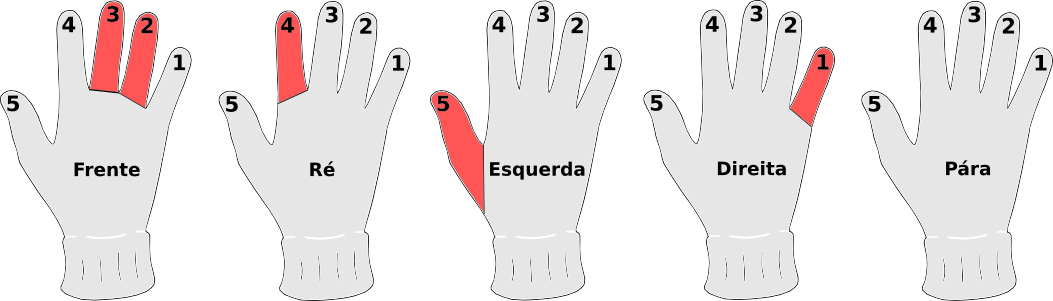
\includegraphics[width=14cm]{./figures/glove-control-positions1.png}
  		\label{Fig:glove-control-positions1}
			\fonte{Produzido pelo autor.}
		\end{figure}

		
		\subsection{\textit{Software} de recepção}

		A biblioteca VirtualWire também deve estar presente no código do microcontrolador embarcado no carrinho. Para receber as mensagens adequadamente, é necessário definir o pino do receptor RF e indicar a taxa de transmissão do transmissor RF. Também deve-se criar variáveis para guardar a mensagem recebida e o seu tamanho, pois as mensagens são recebidas \textit{byte} a \textit{byte}.

		Uma função nativa da biblioteca verifica se chegou alguma mensagem e indica \textit{true} quando isso acontece. Então, ao receber uma mensagem, para lê-la, é necessário criar um \textit{for} que recebe como parâmetro o tamanho da mensagem recebida. Dentro da função a mensagem será lida \textit{byte} a \textit{byte} enquanto a função \textit{for} for verdadeira.

		O pseudocódigo abaixo demonstra o fluxo descrito:


\begin{lstlisting}
	// Define as variaveis
	int pino_receptor = 8;
	int taxa_transmissao = 2000;
	
	// Recebe a mensagem e o seu tamanho
	byte msg = get_mensagem;
	byte tamanho_msg = get_tamanho_msg;
	
	// Aguarda receber alguma mensagem
	chegou_mensagem = vw_wait_rx();

	// Verifica se ha mensagem, inicia o for para ler cada byte
	if(chegou_mensagem){
		for (int i = 0; enquanto i < tamanho_msg; i++)
			byte_recebido[i] = msg[i];		
	}
\end{lstlisting}

		Usando o pseudocódigo apresentado e sabendo que na mensagem recebida o primeiro dígito indica a posição atual do dedo 1, percebe-se que a função \textit{for} irá rodar pelo menos 5 vezes, armazenando em cada posição do vetor \texttt{byte\_recebido[]} as informações de cada dedo. Dessa maneira, a posição recebida do dedo 1 estará em \texttt{byte\_recebido[0]}, enquanto que a do dedo 2 está em \texttt{byte\_recebido[1]}. Continuando assim até o dedo 5 que estará em \texttt{byte\_recebido[4]}.
		
		Após o armazenamento das posições dos dedos, cinco funções foram criadas para comandar a ponte H e dessa forma movimentar os motores do carrinho. São elas: FRENTE( ), TRAS( ), ESQUERDA( ), DIREITA( ) e PARA( ). Ao chamar qualquer uma dessas funções, o carrinho passa a se movimentar na direção e sentido definidas.
		Para chamar a função correta baseada na mensagem recebida, foram criadas cadeias de \textit{Ifs} e \textit{Elses} nas quais, quando satisfeitas certas condições, a respectiva função é chamada. 
		
		A tabela \ref{Tab:dedos-e-comandos1} mostra quais são os conjuntos de valores esperados para todos os dedos simultaneamente em cada comando. Ou seja, para saber qual a combinação de valores para movimentar o carrinho para frente, é só observar a coluna "Frente" da tabela. Qualquer outra combinação além das especificadas na tabela, fará o carrinho ficar parado. Os dedos flexionados estão destacados em vermelho.

		\begin{table}[H]
     \centering
     \caption{Valores recebidos dos dedos e comandos de movimento}
     \begin{tabular}{c|ccccc}
			 \midrule
			 Dedo &       Frente			 & 				Tras				& 		Esquerda			 & 		Direita					& Para	\\
			 \midrule
			 1    & < 2   						 & < 2   							& < 2    						 &\textcolor{red}{> 1}&	-			\\
			 2    &\textcolor{red}{> 1}& < 2   							& < 2  	 						 & < 2   							&	-			\\
			 3    &\textcolor{red}{> 3}& < 4   							& < 4   						 & < 4   							&	-			\\
			 4    & < 4   						 &\textcolor{red}{> 3}& < 4 							 & < 4   							&	-			\\
			 5    & < 5   						 & < 5   							&\textcolor{red}{> 4}& < 5   							&	-			\\
			 \midrule
     \end{tabular}
     \label{Tab:dedos-e-comandos1}
     \fonte{Produzido pelo autor}
   \end{table}



%		Para poder controlar o carrinho, foi necessário criar um protocolo de comunicação que traduzisse os movimentos de flexão dos dedos em comandos e direções para o carrinho que receberia o sinal.


		\section{Assembling}

		\subsection{Transdutor de Flexão}

		A escolha de materiais foi baseada no menor custo e maior disponibilidade local. Prevendo a possibilidade de costuras no projeto, um par de luvas de algodão foi escolhida. O sistema foi embarcado na luva direita, enquanto que a esquerda poderia ser usada em caso de dano da primeira.
		
		As polias plásticas são feitas a partir de pequenos pedaços de hastes flexíveis com algodão nas pontas. Sendo que apenas a parte plástica foi aproveitada enquanto que o algodão foi descartado.

		O material da linha que movimenta os cursores dos potenciômetro é náilon. Isso porque, nos testes, ela apresentou boa resistência e durabilidade, além de aparentar ter pouca ou nenhuma elasticidade para a aplicação.

		Utilizando a luva escolhida com o dorso voltado para cima, as polias plásticas foram costuradas ao longo dos dedos. Uma das extremidades de cada fio de náilon foi presa na ponta de cada um dos dedos, enquanto que o restante do fio passava por dentro das polias plásticas. A outra extremidade do fio de náilon seria amarrada ao cursor do potenciômetro quando a PCB fosse incluída na luva. A figura \ref{Fig:glove-wire-pot1} demostra o resultado esperado para um dos dedos da luva.


		\begin{figure}[h!]
			\centering
			\caption{Costura do transdutor em um dedo.}
  		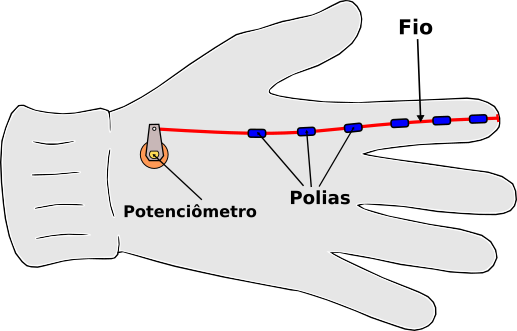
\includegraphics[width=7cm]{./figures/glove-wire-pot1.png}
  		\label{Fig:glove-wire-pot1}
			\fonte{Produzido pelo autor.}
		\end{figure}

			
			\subsection{Escolha de componentes}	

			O sistema de processamento e transmissão de sinal embarcado na luva, foi projetado para ser móvel, leve, alimentado por uma bateria, caber no dorso da mão e ter custo relativamente menor em relação à soluções com sensores flex tradicionais. O sistema dever ser de fácil reprodução e o mais adaptável possível à outras formas de transmissão além da rádio frequência, caso estas sejam necessárias futuramente.

			O primeiro desafio foi escolher, dentre os componentes disponíveis, quais seriam utilizados para compor a eletrônica presente na placa de circuito impresso que estaria embarcada na luva.

			O potenciômetro foi o primeiro componente a ser definido. Isso porque, este seria o componente  em maior número na placa. O modelo escolhido deveria ser pequeno suficiente para manter uma distância adequada para outros potenciômetros e componentes. Seu cursor deveria ser de fácil giro, para que pudesse ser acionado apenas pelo deslocamento do fio. Seu ângulo de giro total precisava ser mínimo, para que o menor grau de giro correspondesse à maior variação de resistência possível, facilitando assim a percepção pelo microcontrolador.

			O modelo de potenciômetro que mais se aproximou das especificações acima foi retirado de servomotores modelo MG996R da marca TowerPro. O potenciômetro encontrado possui dimensão aproximada de 13$mm$ x 13$mm$, resistência máxima de 5k$\Omega$, giro máximo de $200^{o}$ (aproximado) e oferece pouca resistência para girar seu cursor. 

			Um pequeno pedaço de PVC (\textit{Polyvinyl Chloride}) expandido foi adaptado ao cursor do potenciômetro para facilitar o seu giro, amarrar uma das extremidades do fio de náilon e para prender um elástico. Essa adaptação pode ser vista na figura \ref{Fig:potentiometer-and-battery} (a).

			O microcontrolador escolhido para processar os dados recebidos de cada potenciômetro foi o Arduíno modelo Nano. Isso porque ele é leve, ocupa uma área de apenas 45$mm$ x 17$mm$, possui vasta documentação e disponibilidade no mercado, além de ser compatível com diversos módulos externos e possuir custo menor do que outros modelos da família Arduino.

			Para transmitir e receber o sinal, foi escolhido o par de RF 433$Mhz$, que é leve e de baixo custo comparado à outras soluções de transmissão de dados.

			Finalmente, para alimentar esse aparato eletrônico, foi escolhida uma pequena bateria LiPo (\textit{Lithium-ion Polymer}) que possui capacidade de 300$mAh$, 7.4$V$ de tensão nominal e ocupa um espaço de 45$mm$ x 12.5$mm$. Esse modelo é mostrado na figura \ref{Fig:potentiometer-and-battery} (b).


	\begin{figure}[!htb]
		 \centering
		 \caption{ (a) Potenciômetro adaptado e (b) bateria.}
		 \subfloat[]
		 {
			 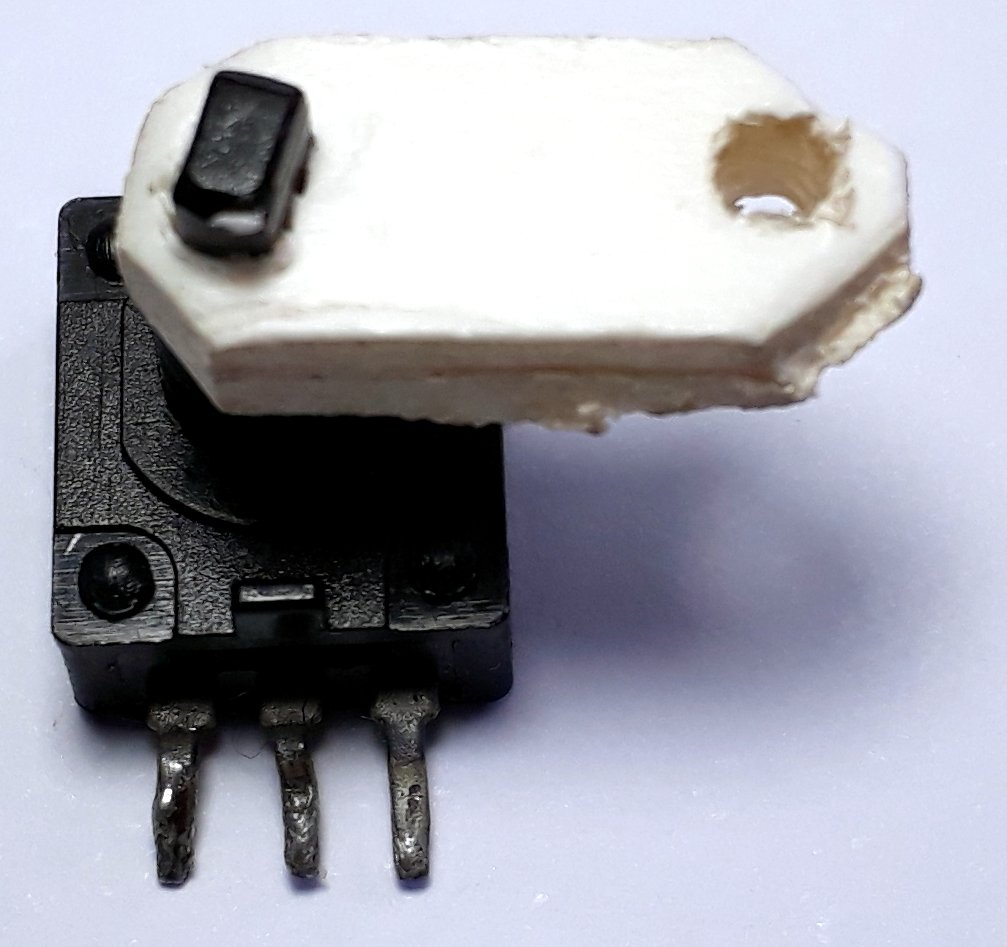
\includegraphics[width=5.5cm,keepaspectratio=true]{./figures/potentiometer3.jpg}
		 }
		 \centering
		 \subfloat[]
		 { 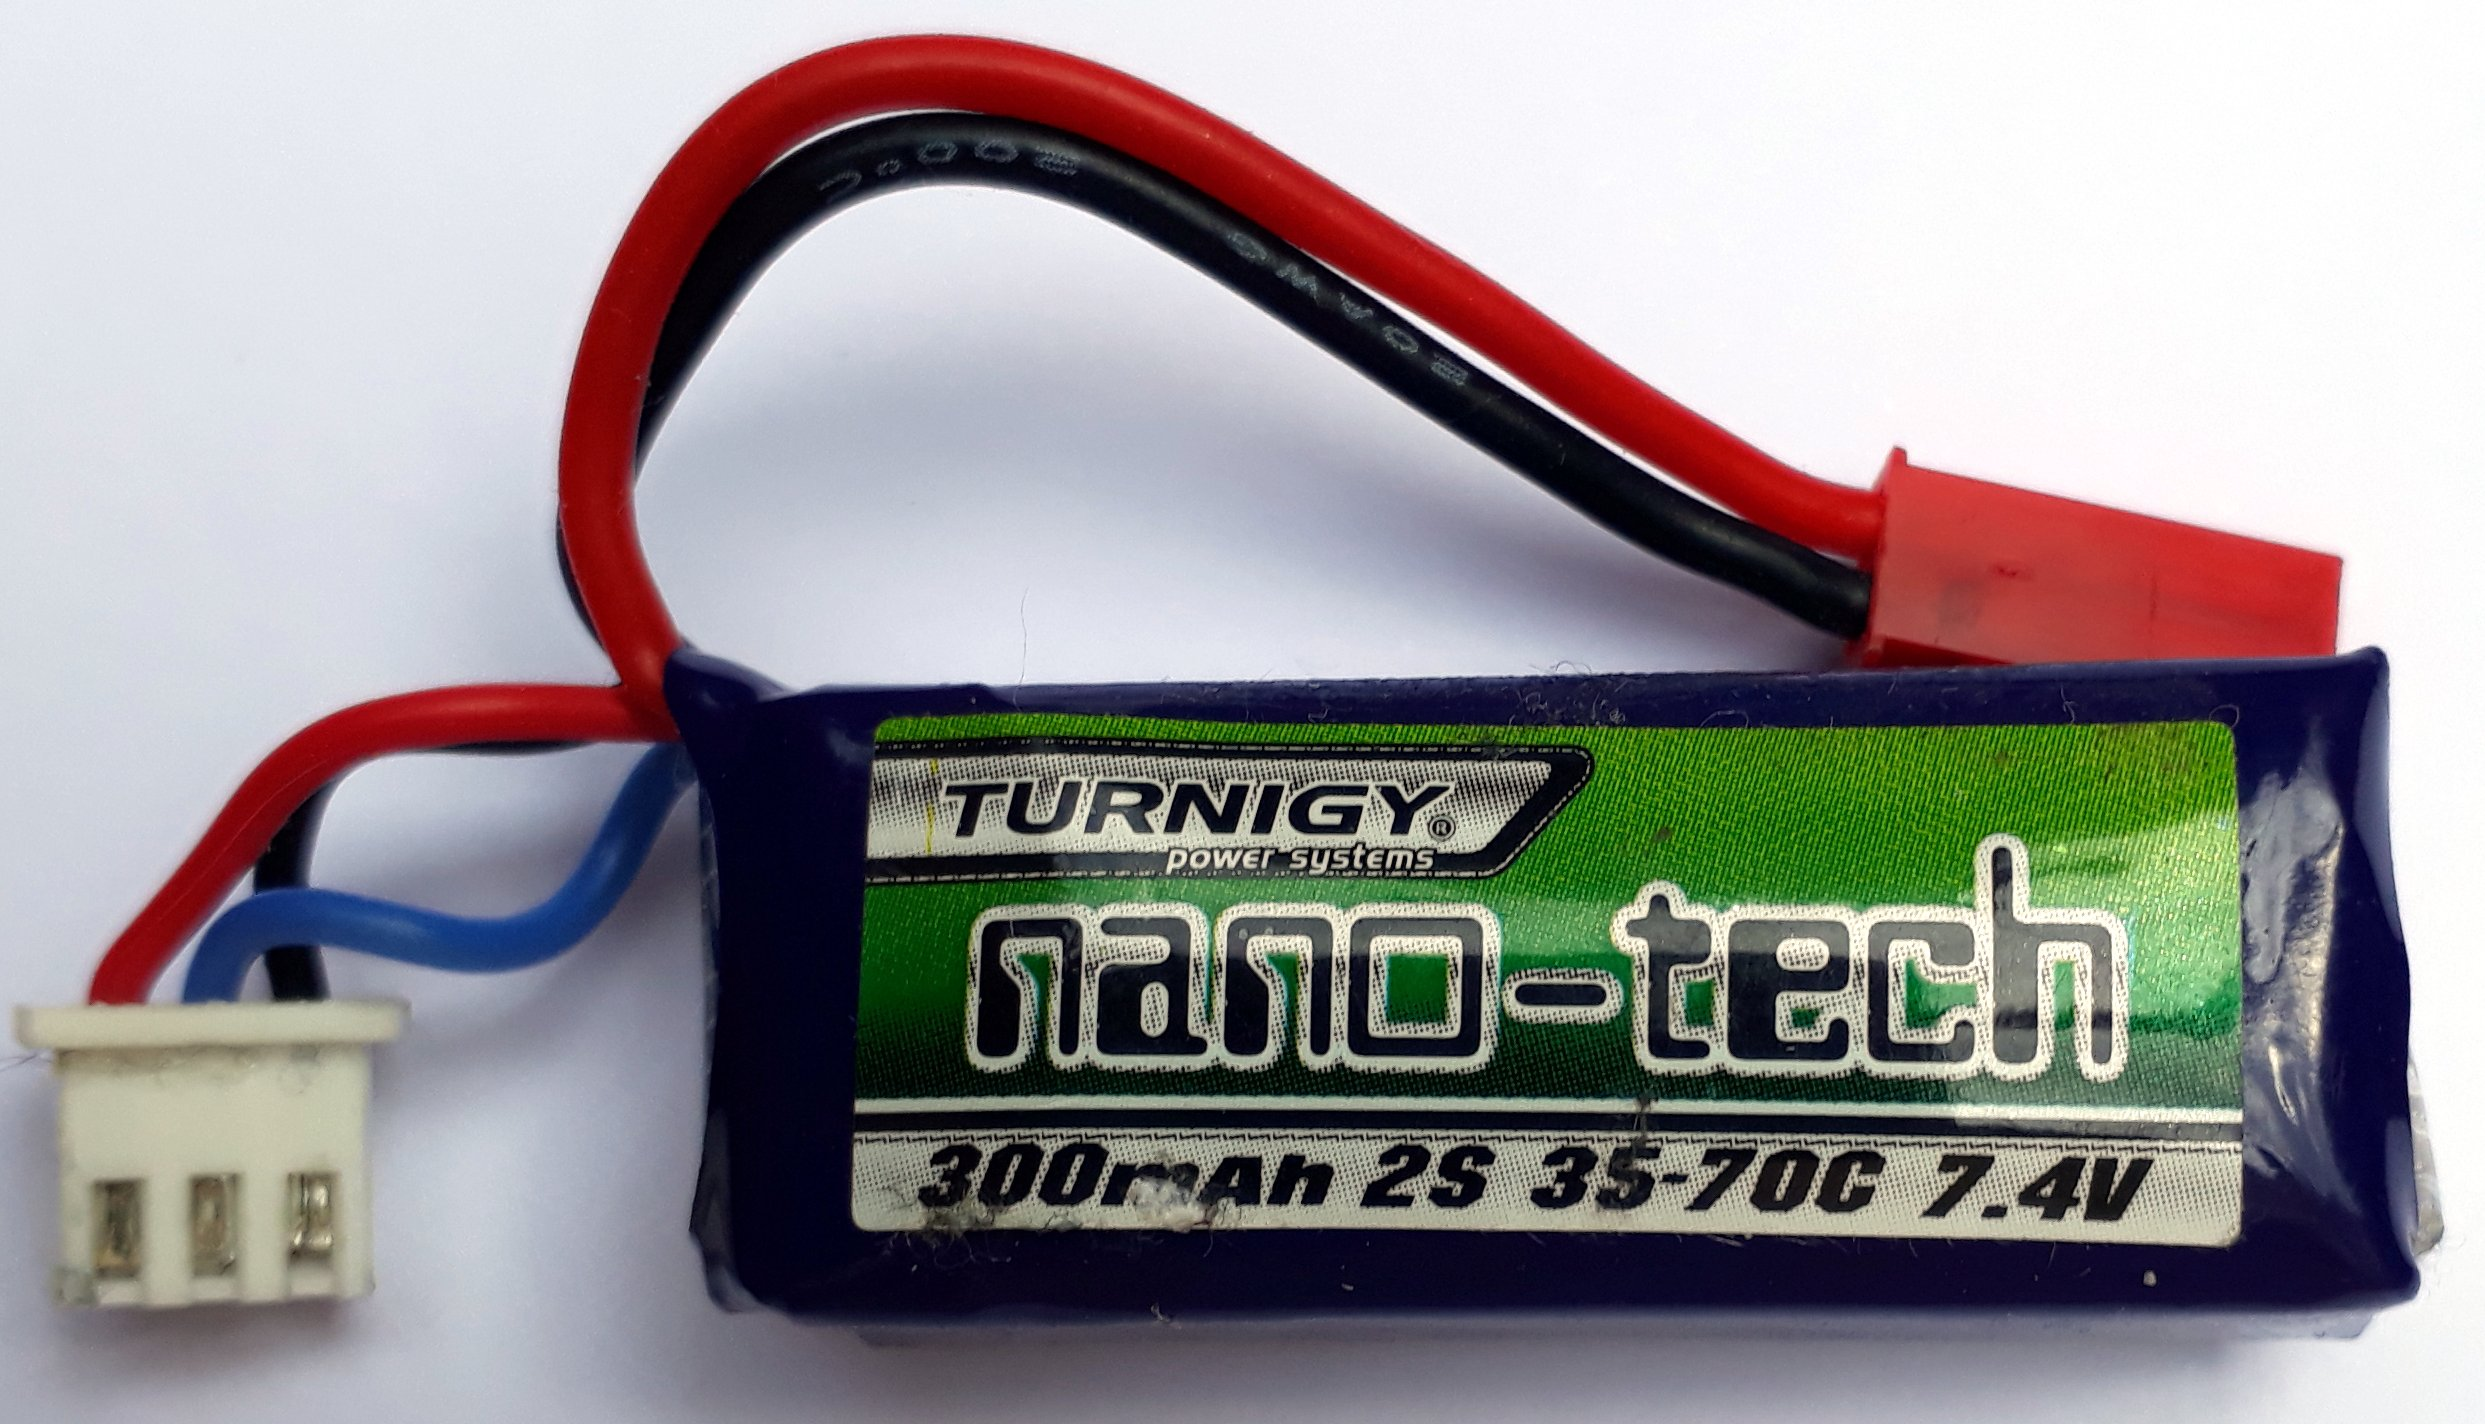
\includegraphics[width=8.5cm,keepaspectratio=true]{./figures/battery1.jpg}
		 }
		 \label{Fig:potentiometer-and-battery}
		 \fonte{Produzido pelo autor.}
	 \end{figure}


			\subsection{Posicionamento de componentes}

			Após medições realizadas na luva que serviu de modelo para o projeto, foi decidido que a dimensão máxima da PCI (Placa de Circuito Impresso) deveria ser de aproximadamente 72$mm$ x 58$mm$. Isso para que a placa não ficasse muito maior do que o dorso da luva. Sendo assim, usando o software QCAD, que é gratuito para os sistemas Linux, todos os componentes foram organizados dentro da placa baseados em suas dimensões aproximadas. Chegando ao \textit{layout} mostrado na figura \ref{Fig:size-glove-module1}.

		\begin{figure}[h!]
			\centering
			\caption{Dimensões aproximadas da PCI e seus componentes.}
  		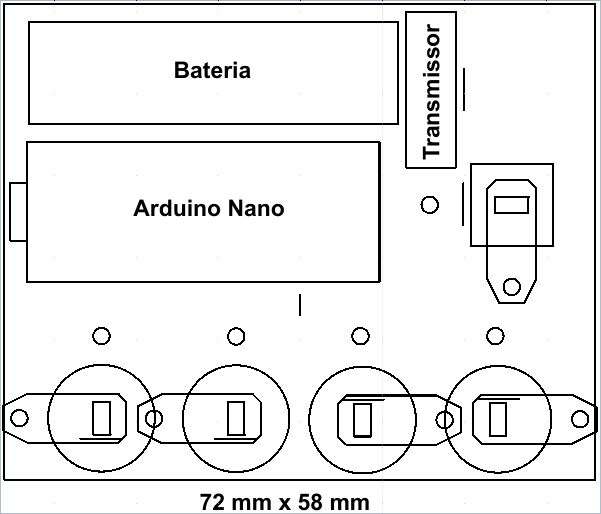
\includegraphics[width=7cm]{figures/size-glove-module1.png}
  		\label{Fig:size-glove-module1}
			\fonte{Produzido pelo autor.}
		\end{figure}


			\subsection{Placa Embarcada}

			Os primeiros experimentos de ligação e testes entre os componentes foram realizados ainda em protoborad. Inicialmente, um simples programa lia a variação de um resistor e mostrava na tela do computador. Este e outros programas foram usados para verificar como deveriam ser as conexões entre os pinos, potenciômetros, bateria, módulo transmissor e o microcontrolador Arduíno.

			O passo seguinte foi utilizar o software gratuito Kicad para desenhar o esquemático da placa. Posteriormente, o Kicad ainda possibilita projetar uma placa de circuito impresso baseada no esquemático desenhado anteriormente. Através desse software foram criados os desenhos do esquemático e da PCI embarcada mostrados na figura \ref{Fig:schematic-and-PCB}.

	\begin{figure}[!htb]
		 \centering
		 \caption{ Desenhos projetados no Kicad do (a) esquemático e (b) PCI. }
		 \subfloat[]
		 {
			 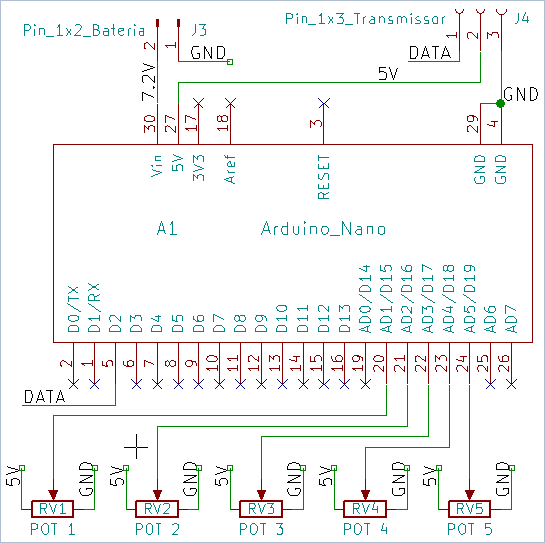
\includegraphics[width=6.5cm,keepaspectratio=true]{./figures/schematic-glove-module1.png}
		 }
		 \centering
		 \subfloat[]
		 { 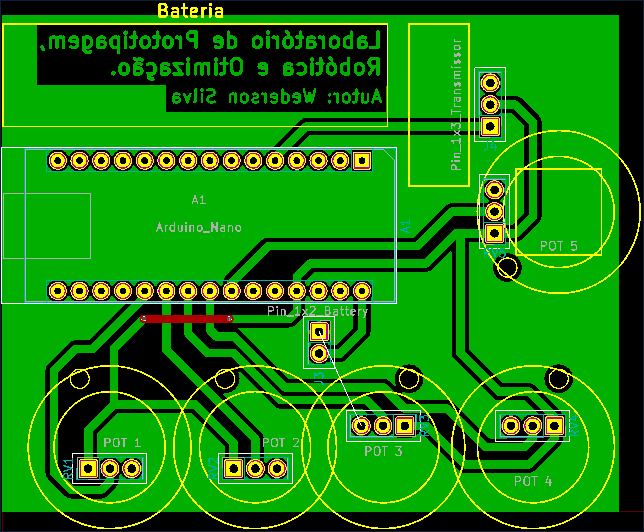
\includegraphics[width=7.5cm,keepaspectratio=true]{./figures/PCB-glove-module1.png}
		 }
		 \label{Fig:schematic-and-PCB}
		 \fonte{Produzido pelo autor.}
	\end{figure}

			Após a conclusão do desenho da placa, foram efetuados os procedimentos necessários para a confecção desta PCI em uma placa de fenolite cobreada, além da posterior soldagem de pinos e componentes. A figura \ref{Fig:phenolic-and-ready} mostra os resultados após o procedimento descrito. Já a figura \ref{Fig:glove-ready1} mostra o resultado final após juntar a luva de algodão e a placa de circuito impresso recém concluída.

	\begin{figure}[!htb]
		 \centering
		 \caption{(a) Placa de fenolite cobreada e (b) com os componentes soldados.} 
		 \subfloat[]
		 {
			 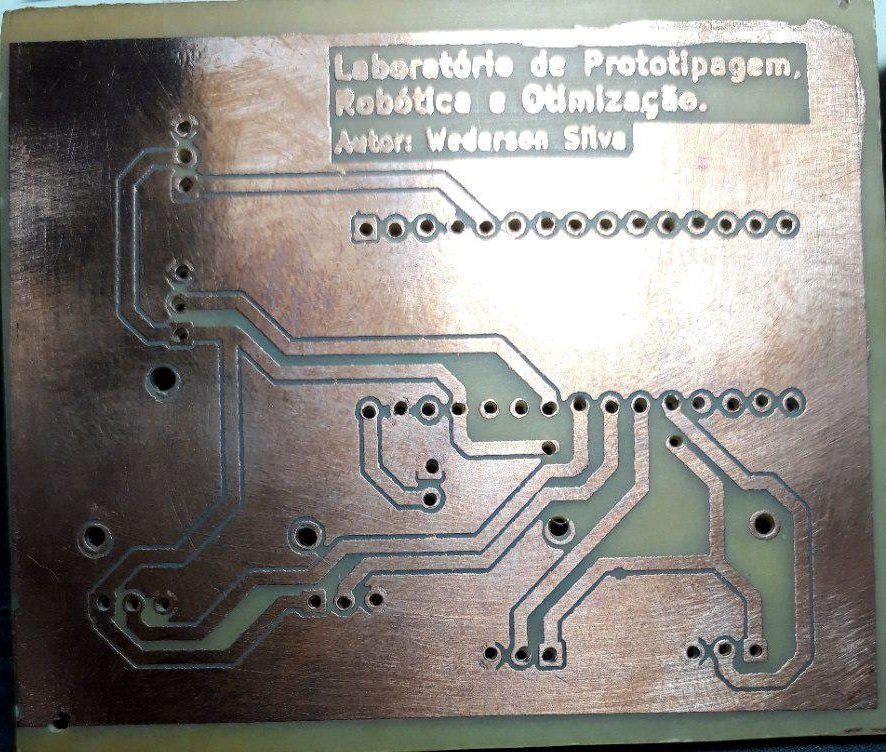
\includegraphics[width=7cm,keepaspectratio=true]{./figures/phenolic-glove-module1.jpg}
		 }
		 \centering
		 \subfloat[]
		 { 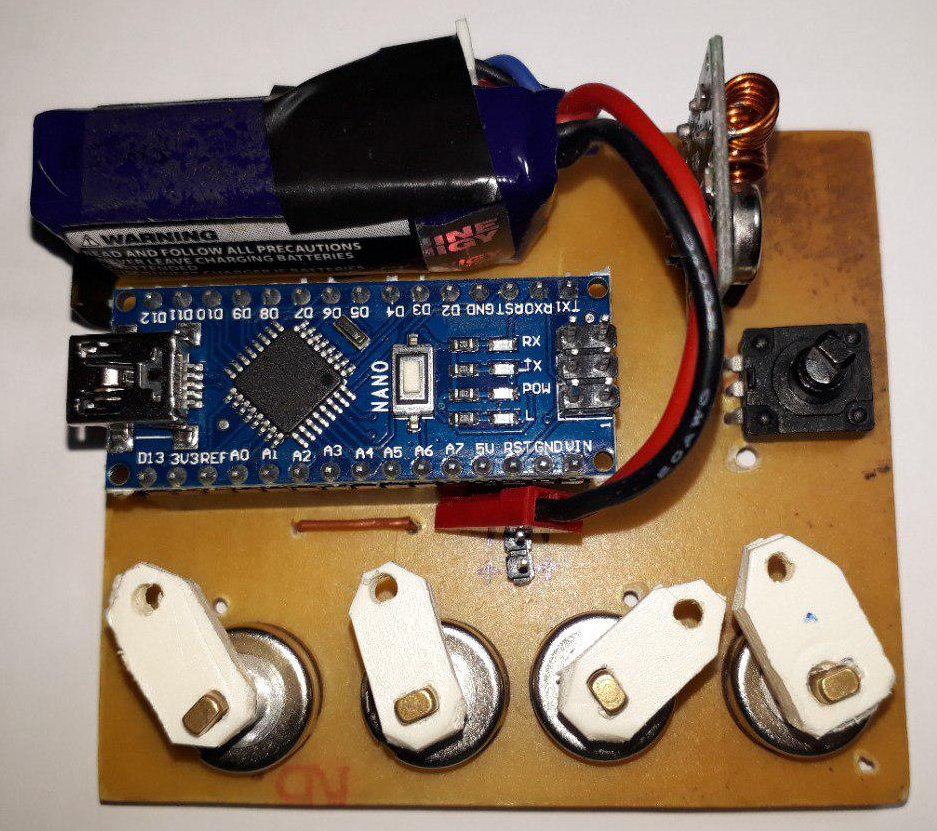
\includegraphics[width=7cm,keepaspectratio=true]{./figures/glove-module-ready1.jpg}
		 }
		 \label{Fig:phenolic-and-ready}
		 \fonte{Produzido pelo autor.}
	\end{figure}

%		\section{Montagem}

%		Utilizando uma luva de algodão, em seu dorso foi costurado uma das metades de um pedaço de velcro (gancho) de dimensões semelhantes à PCI contruída anteriormente. Ao longo dos dedos da luva foram costurados pequenos segmentos de plástico que serviriam como guias para os fios.	Na parte inferior da PCI foi costurada a outra metade do velcro (argola) que poderia ser fixada, sempre que fosse preciso, à outra parte do velcro costurada na luva.

%		Fios de náilon foram fixados nos segmentos de plástico (guias) localizados nas pontas dos dedos da luva. Os fios passavam por dentro das guias até serem amarrados em pequenos pedaços de PCV expandido que estavam conectados dos cursores dos potenciômetros. Por fim, pequenos pedaços de elástico, levemente esticados, também foram amarrados nos pedaços de PCV expandido.
		

		\begin{figure}[h!]
			\centering
			\caption{Luva montada.}
  		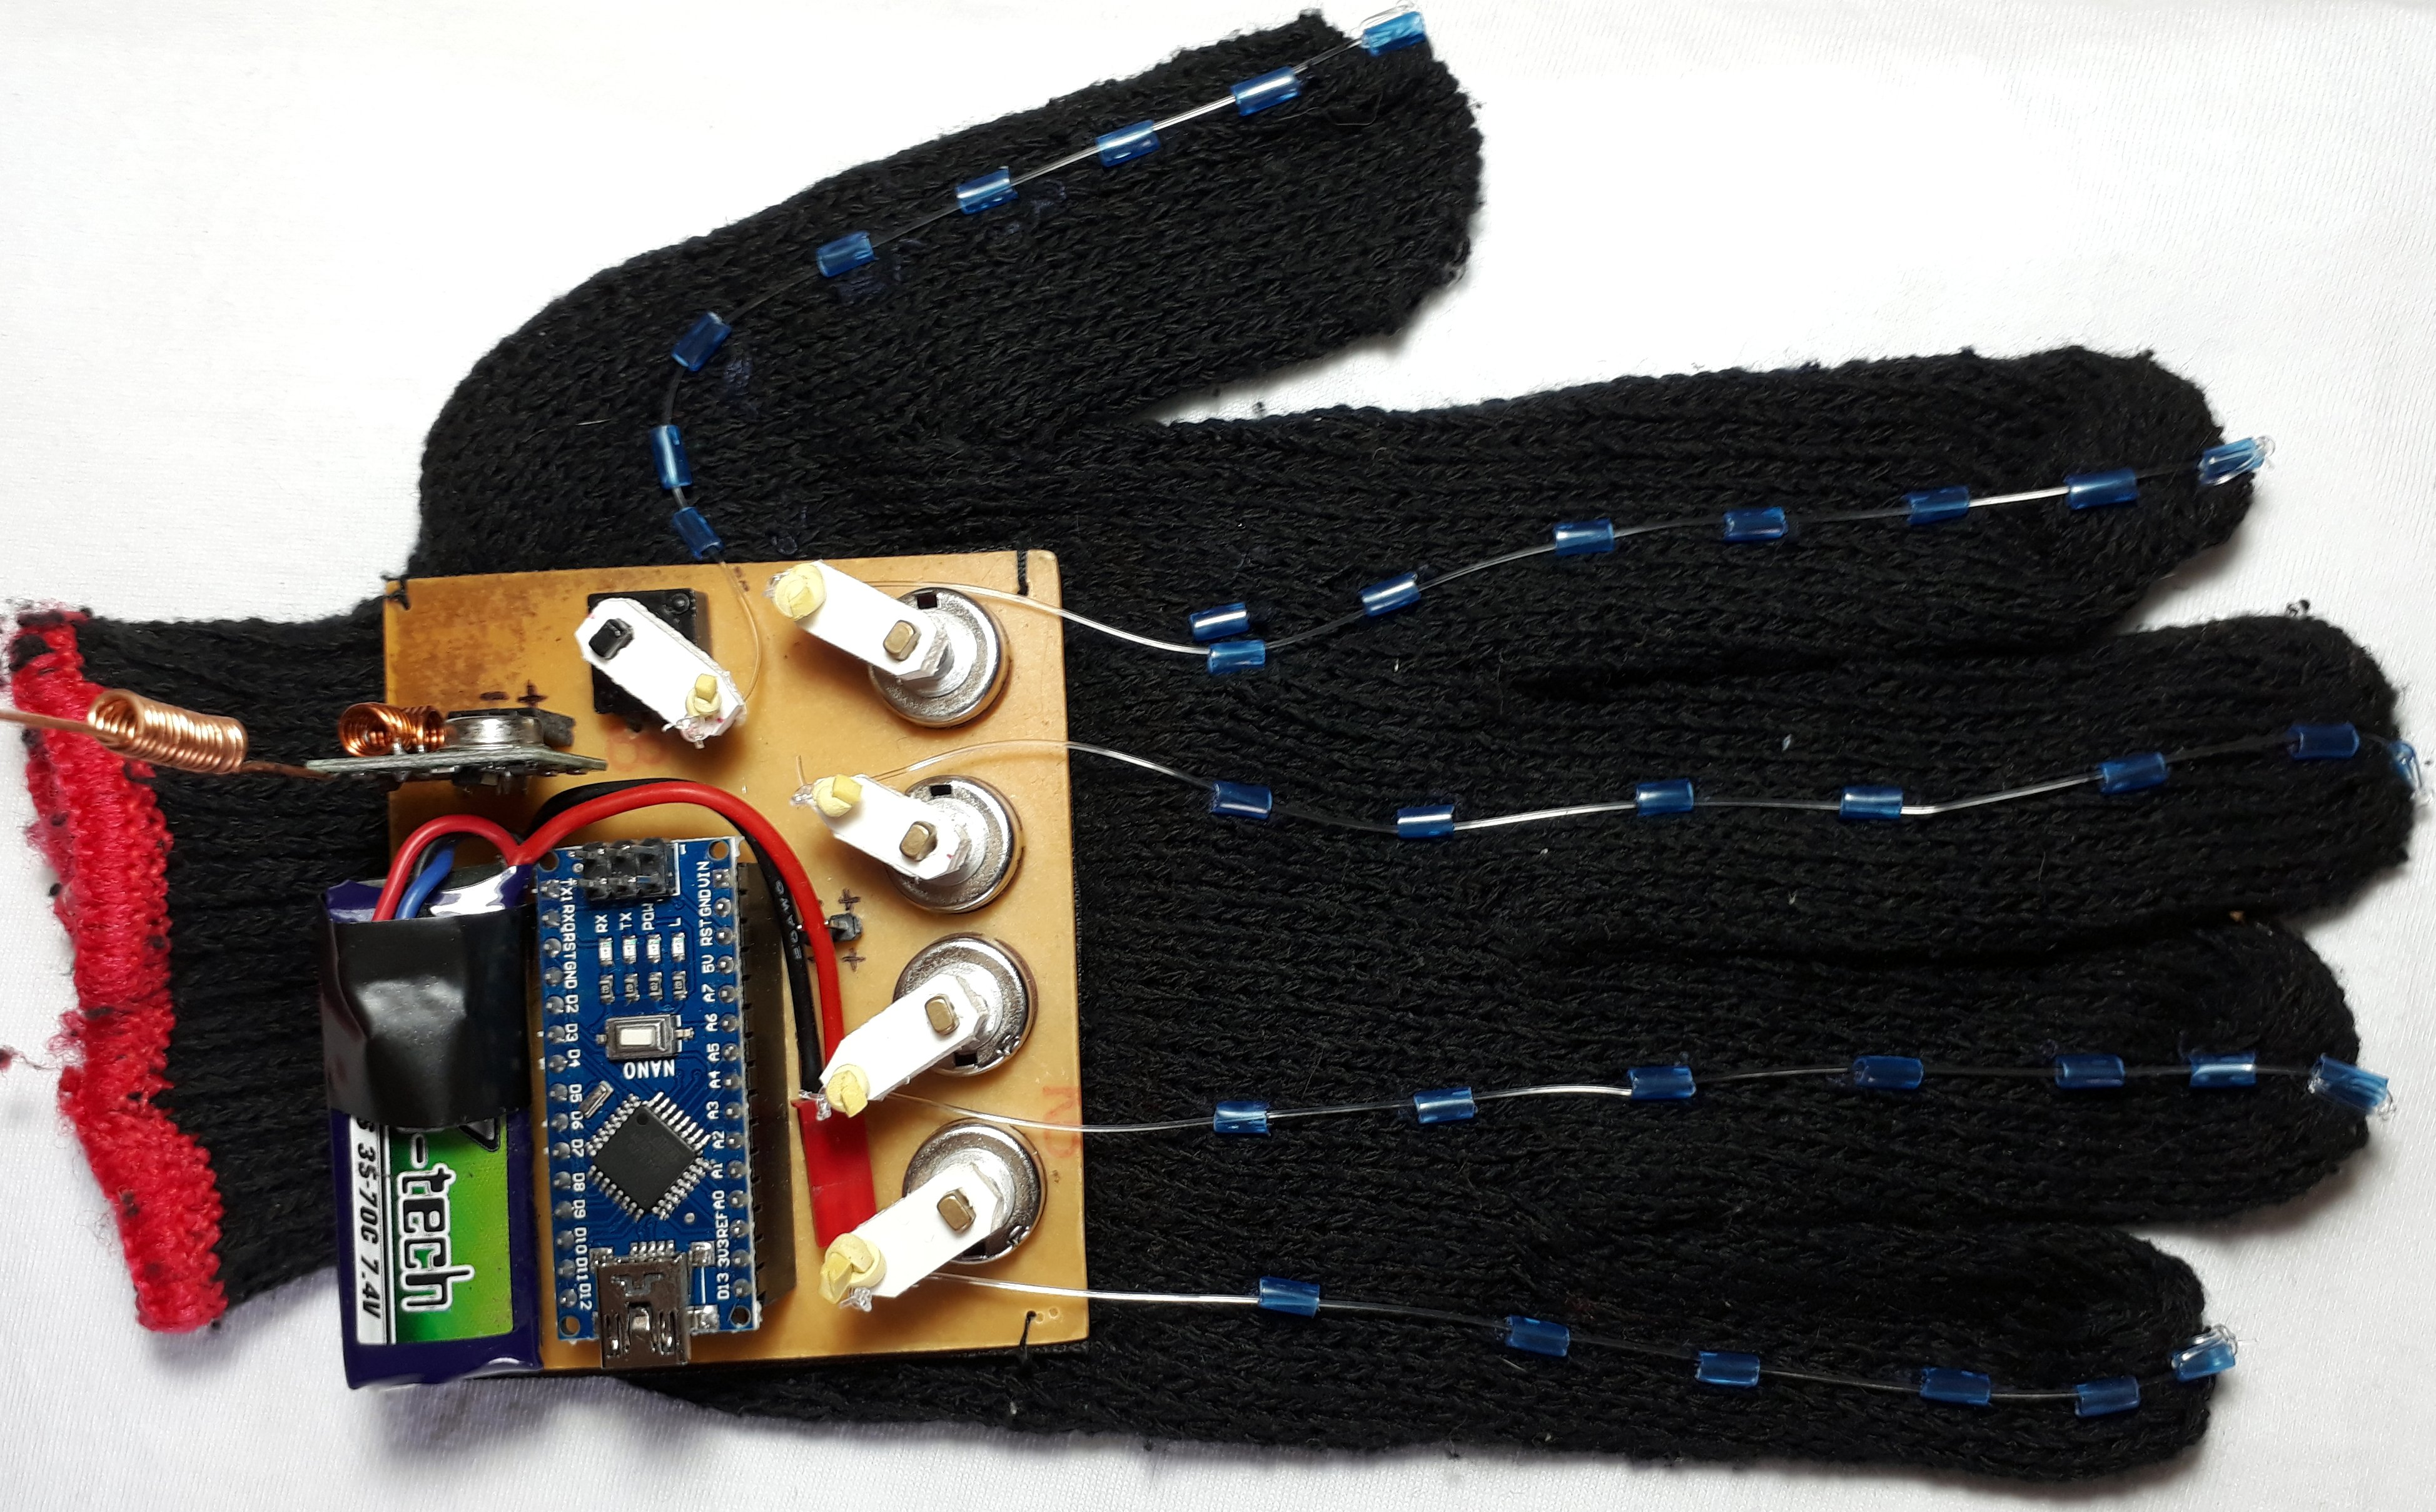
\includegraphics[width=14cm,keepaspectratio=true]{figures/glove-ready1.jpg}
  		\label{Fig:glove-ready1}
			\fonte{Produzido pelo autor.}
		\end{figure}


		

		\chapter{BUFFER}
		Também é possível notar que alguns deslocamentos são positivos enquanto outros são negativos. Isso se dá porque os potênciometros 1 e 2 foram instalados com seus cursores em sentido oposto aos potenciômetros 3 e 4. Com o intuito de minimizar o espaço entre eles na placa. Isso pode ser observado na figura \ref{Fig:glove-ready1}.

		Por conta desse fato, durante o movimento de flexão, os potenciômetros 1 e 2 giram em sentido anti-horário e possuem deslocamento positivo, enquanto os demais giram em sentido horário com deslocamento negativo. No caso do potenciômetro 5, apesar de girar em sentido anti-horário, ele possui um deslocamento negativo. Isso porque foi soldado em posição reversa aos demais, com o propósito de maximar sua aderência na placa.




		\section{Transmissão e Recepção de Dados}

			Como foi descrito, durante a movimentação dos dedos, a posição do cursor do potenciômetro é modificado. Sendo assim, para possibilitar o sensoriamento, a variação de cada potenciômetro é captada por um microcontrolador que processa esse sinal antes de despachá-lo para o transmissor. Este por sua vez envia mensagens por rádio frequência, em formato de números inteiros que representam a posição atual de cada dedo. Figura \ref{Fig:transmitter-and-receptor} (a).

			O módulo receptor de rádio frequência, capta as mensagens e as envia a outro microcontrolador. Este por sua vez, processa a mensagem e transmite aos respectivos componentes e atuadores daquela aplicação. Figura \ref{Fig:transmitter-and-receptor} (b).


	\begin{figure}[!htb]
  	\centering
   	\caption{ (a) Transmissão do sinal. (b) Recepção do sinal.}
   	\subfloat[]
   	{
     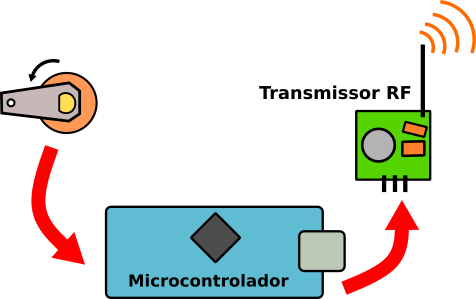
\includegraphics[width=7cm,keepaspectratio=true]{./figures/transmitter-module1.png}
    }
   	\centering
   	\subfloat[]
   	{ 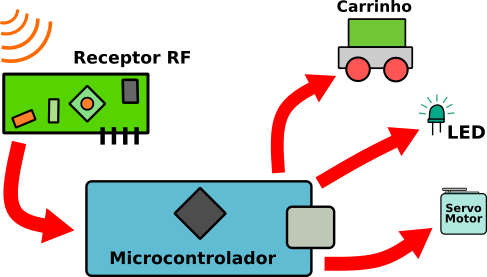
\includegraphics[width=7cm,keepaspectratio=true]{./figures/receptor-module1.png}
   	}
   	\label{Fig:transmitter-and-receptor}
   	\fonte{Produzido pelo autor.}
 		\end{figure}


			Para este trabalho, um pequeno carrinho, foi o sistema escolhido para ser controlado pela luva. Para isso, um protocolo de transmissão foi desenvolvido para traduzir os movimentos dos dedos da luva em direções para o carrinho.


	
		
		

	% ----------------------------
	%	RESULTADOS E ANÁLISES	
	% ----------------------------
	
	\chapter{Análises e Resultados}

		\section{Configurações}

		\section{Testes}

		\section{Resultados}
		

	% ----------
	%	CONCLUSÃO	
	% ----------
  \chapter{Conclusão}

		\section{Conclusões}

		\section{Trabalhos Futuros}


% ----------------------------------------------------------
% ELEMENTOS PÓS-TEXTUAIS
% ----------------------------------------------------------
\postextual
% ----------------------------------------------------------
% Referências bibliográficas
% ----------------------------------------------------------
\bibliography{referencias}

%---------------------------------------------------------------------
% INDICE REMISSIVO
%---------------------------------------------------------------------

\printindex

\end{document}
